% ============================================================================
% Bioinspiration & Biomimetics — IOP Publishing
% Compile on Overleaf using the IOP template:
%   https://www.overleaf.com/latex/templates/template-for-iop-publishing-journals/dbftskdgszdz
% Download iopart.cls from IOP if compiling locally.
%
% If iopart.cls is unavailable, change the line below to:
%   \documentclass[12pt]{article}
% and comment out the \submitto and \ead lines.
% ============================================================================
\documentclass[12pt]{iopart}

\usepackage{graphicx}
\graphicspath{{figures/}}
\usepackage{amsmath,amssymb}
\usepackage{booktabs}
\usepackage{hyperref}
\usepackage[caption=false]{subfig}
\usepackage{array}
\usepackage{tabularx}
\usepackage{mathtools}

% Ensure \BB is defined (journal abbreviation for iopart \submitto)
\providecommand{\BB}{\textit{Bioinspir. Biomim.}}

\begin{document}

\title{Scaffolding Dynamic Leader-Follower Coordination in Swarm Robotics through Constraint Closure and Multi-Timescale Social Interactions}

\author{Pranay Vaddepalli$^{1}$, Fethi Candan$^{1}$ and Alejandro Jimenez Rodriguez$^{1}$}

\address{$^{1}$ Department of Computer Science, University of South Florida, Tampa, FL, USA}

\ead{ajimenez3@usf.edu}

\begin{abstract}
Multi-agent systems face a fundamental stability-plasticity dilemma: maintaining coherent coordination while adapting to environmental disruptions. Biological social groups solve this through \emph{constraint closure}---circular causal loops where individual actions generate group-level constraints that in turn shape future individual behaviour. Whether such mechanisms can scaffold emergent leader-follower coordination in artificial swarms remains an open question.

We present a three-timescale architecture---fast task execution, medium-rate energy dynamics, and slow bond accumulation---validated across 50 independent simulation runs of 10-agent swarms performing a collective foraging task. A geometric state-space decomposition formalises \emph{explicit} and \emph{implicit} pressure channels with no free parameters, directly operationalising Wilson and Prescott's constraint closure framework. A complementary Landau free energy model connects the observed dynamics to established phase transition theory.

Three principal findings emerge. First, circular causality is confirmed through detrended cross-correlation across a four-link causal chain (Success $\to$ Energy $\to$ Grooming $\to$ Bonds), with multi-run validation ($N=50$, lag-10 peak $r = 0.153 \pm 0.016$). Second, channel-specific perturbation response constitutes the paper's most novel contribution: resource scarcity targets the explicit pressure channel while bonds remain buffered ($S_\mathrm{VN}$ stable at ${\sim}0.101$--$0.105$), whereas leader removal targets the implicit channel, triggering structural reorganisation ($S_\mathrm{VN}$: $0.101 \to 0.085 \to 0.151$). The system shows minimal degradation under extreme perturbation (0.9--2.3\% immediate performance loss), with distinct thermodynamic recovery signatures depending on perturbation type. Third, bidirectional causal symmetry is established through controlled average treatment effect analysis with Cohen's $d$ normalisation, collapsing an apparent $870\times$ asymmetry in raw Granger statistics to approximate parity: individual behaviour is more \emph{efficient} per unit intervention ($d \approx 1.7$--$2.2$), while the group exerts more \emph{total force} ($d \approx 1.2$--$1.6$). Scalability analysis identifies a coordination limit at 10--12 agents, paralleling grooming bandwidth constraints observed in primate social groups.
\end{abstract}

% PACS/keywords
\submitto{\BB}

\maketitle

%==============================================================================
\section{Introduction}
\label{sec:intro}
%==============================================================================

Catastrophic forgetting---the tendency for learned capabilities to degrade when agents encounter novel situations---remains a central challenge in multi-agent reinforcement learning \cite{mccloskey1989,kirkpatrick2017}. When coordination strategies acquired under stable conditions encounter environmental disruptions, performance often collapses irreversibly. This stability-plasticity dilemma demands architectures that preserve functional competence while permitting adaptive reorganisation \cite{parisi2019}.

Biological social groups offer a compelling solution. Baboon troops, for instance, maintain coherent group coordination despite continuous membership changes, resource fluctuations, and predation events \cite{king2009,seyfarth2012}. Their resilience arises not from centralised control but from \emph{constraint closure}: circular causal loops where individual behaviours generate group-level social structures that subsequently constrain individual action \cite{wilson2022}. Wilson and Prescott \cite{wilson2022} formalised this as a dynamic interplay between \emph{explicit} pressures (environmental demands on individuals) and \emph{implicit} pressures (social structural constraints), arguing that the closure of these causal loops scaffolds emergent group-level competence.

Existing multi-agent coordination approaches address aspects of this challenge. Consensus-based methods \cite{olfati2004,ren2005} provide mathematical convergence guarantees but assume static topologies. Market mechanisms \cite{dias2006} enable flexible task allocation but lack the persistent social memory that supports recovery from disruption. Stigmergic approaches \cite{dorigo2004,theraulaz1999} produce emergent coordination through environmental modification but offer limited social complexity. Hierarchical architectures \cite{werger2000,chen2020} impose leader-follower structures by design but cannot model leadership emergence. None of these approaches implements the circular causal architecture that characterises biological social resilience.

This gap motivates our central research question: \emph{Can constraint closure, implemented through multi-timescale social dynamics, scaffold emergent leader-follower coordination that exhibits biologically realistic resilience to environmental perturbation?}

We make five contributions:
\begin{enumerate}
\item A three-timescale simulation architecture with 50-run circular causality validation demonstrating constraint closure through a four-link causal chain.
\item A geometric pressure decomposition with no free parameters that operationalises Wilson and Prescott's explicit/implicit pressure framework, complemented by a Landau free energy model connecting to phase transition theory.
\item Channel-specific perturbation response: perturbations targeting different pressure channels produce distinct thermodynamic recovery signatures, providing a diagnostic framework for predicting system resilience.
\item Bidirectional causal symmetry between individual and group levels, demonstrated through Cohen's $d$-normalised average treatment effects that collapse a raw $870\times$ Granger asymmetry.
\item Scalability limits at 10--12 agents confirmed through systematic group size variation, with ablation studies identifying three essential parameters with distinct mechanistic roles.
\end{enumerate}

The remainder of this paper is organised as follows. Section~\ref{sec:methods} presents the theoretical framework, simulation architecture, and experimental design. Section~\ref{sec:results} reports results across circular causality validation, phase transitions, perturbation response, and causal analysis. Section~\ref{sec:discussion} discusses implications and limitations. Section~\ref{sec:conclusions} concludes.


%==============================================================================
\section{Methods}
\label{sec:methods}
%==============================================================================

\subsection{Theoretical framework}
\label{sec:theory}

\subsubsection{Geometric state-space decomposition.}

We formalise Wilson and Prescott's \cite{wilson2022} pressure concept through a geometric decomposition of the system's state space. The collective state vector $\mathbf{x}(t) = [E(t), B(t), S(t), G(t)]$ captures mean energy~$E$, mean bond strength~$B$, task success rate~$S$, and grooming frequency~$G$ at trial~$t$.

The total system pressure $P_\mathrm{total}$ is decomposed into explicit and implicit components:
\begin{equation}
P_\mathrm{total}(t) = P_\mathrm{explicit}(t) + P_\mathrm{implicit}(t).
\label{eq:ptotal}
\end{equation}

\emph{Explicit pressure} captures environmental demands that individuals experience directly---resource scarcity, task difficulty, and energy costs:
\begin{equation}
P_\mathrm{explicit}(t) = \left\| \frac{\mathrm{d}\mathbf{x}_\mathrm{env}}{\mathrm{d}t} \right\| \cdot \frac{1}{E(t)},
\label{eq:pexplicit}
\end{equation}
where $\mathbf{x}_\mathrm{env} = [E(t), S(t)]$ is the environmentally determined subspace and the energy denominator captures the system's diminishing capacity to absorb further environmental demands as resources deplete.

\emph{Implicit pressure} captures constraints arising from social structure---bond asymmetries, coordination overhead, and emergent role differentiation:
\begin{equation}
P_\mathrm{implicit}(t) = \left\| \frac{\mathrm{d}\mathbf{x}_\mathrm{soc}}{\mathrm{d}t} \right\| \cdot \left(1 - \frac{B(t)}{B_\mathrm{cap}}\right),
\label{eq:pimplicit}
\end{equation}
where $\mathbf{x}_\mathrm{soc} = [B(t), G(t)]$ is the socially determined subspace and the bond capacity term captures how developed social structures buffer against implicit pressure.

The critical insight is the \emph{pressure crossover}: in early dynamics (Phase~I), $P_\mathrm{explicit} > P_\mathrm{implicit}$ as environmental demands dominate; as bonds develop, implicit pressure rises while explicit pressure decreases, crossing at time $t_\mathrm{cross}$ which we identify as the phase boundary:
\begin{equation}
t_\mathrm{cross}: \quad P_\mathrm{explicit}(t_\mathrm{cross}) = P_\mathrm{implicit}(t_\mathrm{cross}).
\label{eq:tcross}
\end{equation}

This decomposition introduces no free parameters---every term is computed directly from simulation observables and the bond capacity parameter $B_\mathrm{cap}$.


\subsubsection{Landau free energy model.}

To connect the observed phase transitions to established thermodynamic theory, we construct a Landau free energy model. We map the bond order parameter $\phi \equiv B/B_\mathrm{cap}$ (normalised mean bond strength) and the system temperature $T \equiv 1/E$ (inverse mean energy, capturing fluctuation intensity) to a free energy functional:
\begin{equation}
F(\phi, T) = a\phi^2 + bT\phi^4,
\label{eq:landau}
\end{equation}
with $a = -0.5$ (favouring the ordered state) and $b = 10^{-6}$ (providing higher-order stabilisation). These coefficients are chosen to capture qualitative phase transition behaviour; they are not fitted to data but selected to place the model in the correct symmetry regime---negative~$a$ ensures the system favours bond formation, while the $T$-dependent quartic term provides a restoring force whose strength scales with thermal fluctuations.

The Landau pressure is derived as:
\begin{equation}
P_\mathrm{Landau} = -\frac{\partial F}{\partial \phi} = -2a\phi - 4bT\phi^3.
\label{eq:plandau}
\end{equation}

When $P_\mathrm{Landau} > 0$, the system is driven toward higher bond order (coordination); when $P_\mathrm{Landau} < 0$, the system experiences pressure toward disorder.

The three pressure frameworks relate as follows. $P_\mathrm{net}$ (see Supplementary Material~S1) quantifies constraint difficulty at the individual agent level through four mechanistic components. The geometric decomposition (equations~(\ref{eq:ptotal})--(\ref{eq:tcross})) formalises Wilson and Prescott's pressure concept at the system level with no free parameters, serving as the primary analytical tool. The Landau model provides thermodynamic predictions connecting to established phase transition theory \cite{landau1980}, particularly valuable as a diagnostic during perturbation analysis where the sign of $P_\mathrm{Landau}$ distinguishes qualitatively different recovery regimes.


\subsubsection{Bond network entropy.}

To characterise the structural complexity of the bond network, we employ the von Neumann entropy of the normalised bond matrix:
\begin{equation}
S_\mathrm{VN} = -\sum_i \mu_i \ln \mu_i,
\label{eq:svn}
\end{equation}
where $\mu_i$ are the eigenvalues of the symmetric bond matrix $\mathbf{A}(t)$ normalised by $\mathrm{tr}(\mathbf{A})$, using only positive eigenvalues for the entropy calculation. Higher $S_\mathrm{VN}$ indicates a more distributed, egalitarian bond topology; lower $S_\mathrm{VN}$ indicates concentrated, hierarchical structure.


\subsection{Simulation architecture}
\label{sec:simulation}

The simulation models $N$ agents (default $N = 10$) performing a collective foraging task over $T = 5000$ trials. Each trial consists of five phases: initiator selection, follower recruitment, task execution, grooming, and energy dynamics.

\begin{figure}[t]
\centering
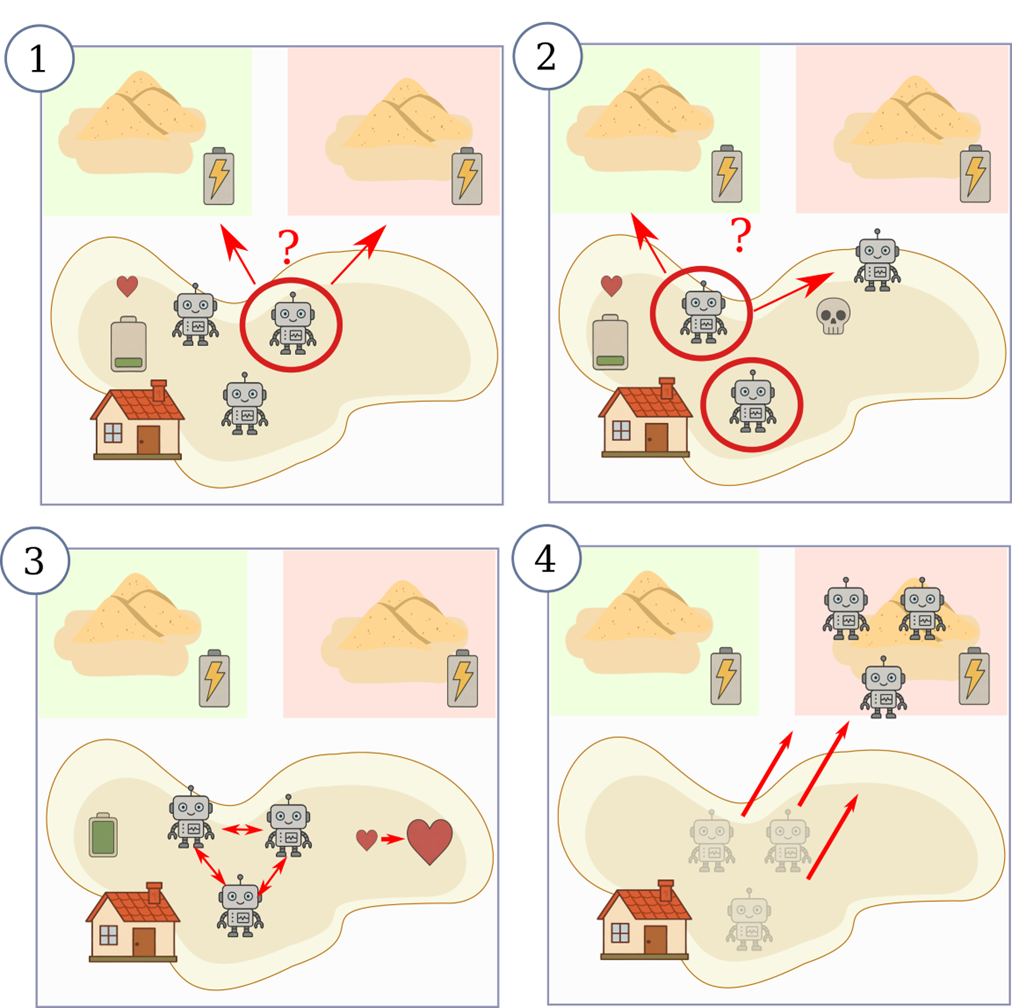
\includegraphics[width=0.8\columnwidth]{simulation.png}
\caption{Task schematic illustrating the four phases of a single trial. (1)~An initiator is selected and decides whether to recruit followers. (2)~Followers decide whether to join based on bond strength. (3)~The group executes the task and engages in grooming. (4)~Successful coordination yields shared energy rewards. Any agent may be selected as initiator, but only those with strong bonds successfully recruit followers---leadership \emph{emerges} from accumulated social bonds.}
\label{fig:schematic}
\end{figure}

Figure~\ref{fig:schematic} illustrates the task schematic. An \emph{initiator}~$l$ is selected uniformly at random from active agents (those with energy $E_i > 0$). We distinguish \emph{initiation} (random focal agent selection) from \emph{leadership} (emergent influence from accumulated bonds): any agent may be selected as initiator, but only those with strong bonds successfully recruit followers.

The initiator decides whether to attempt group coordination with probability:
\begin{equation}
P_\mathrm{init}(l) = \sigma\!\left(\alpha_1 \cdot \frac{E_l}{E_\mathrm{max}} + \alpha_2 \cdot \frac{\bar{A}_l}{A_\mathrm{max}} + \alpha_3 \cdot r_{\mathrm{success},l}\right),
\label{eq:pinit}
\end{equation}
where $\sigma$ is the sigmoid function, $E_l$ is the initiator's energy, $\bar{A}_l$ is their mean bond strength, $r_{\mathrm{success},l}$ is their recent success rate, and $\alpha_1, \alpha_2, \alpha_3$ are weighting coefficients.

Each potential follower~$j$ decides whether to follow initiator~$l$ based on:
\begin{equation}
P_\mathrm{follow}(j, l) = \sigma\!\left(\beta_1 \cdot \frac{A_{jl}}{A_\mathrm{max}} + \beta_2 \cdot \frac{E_j}{E_\mathrm{max}} + \beta_3 \cdot (1 - r_{\mathrm{recent},j})\right),
\label{eq:pfollow}
\end{equation}
where $A_{jl}$ is the bond strength between~$j$ and~$l$, $E_j$ is the follower's energy, $r_{\mathrm{recent},j}$ is their recent success rate, and $\beta_1, \beta_2, \beta_3$ are weighting coefficients.

Task success depends on group size, with a minimum threshold for coordination benefit. Successful group coordination yields energy rewards shared among participants. After task completion, agents engage in grooming---a bond-strengthening interaction:
\begin{equation}
A_{ij}(t+1) = \begin{cases} \min(B_\mathrm{cap},\; A_{ij}(t) + \delta_A) & \text{if grooming}(i,j) \text{ at trial } t, \\ A_{ij}(t) & \text{otherwise,} \end{cases}
\label{eq:bondupdate}
\end{equation}
where $B_\mathrm{cap}$ is the bond capacity (default 200) and $\delta_A = 0.2$ is the grooming increment. Energy decays by a basal metabolism cost each trial. Full algorithmic details, including the grooming decision process and energy dynamics, are provided in Supplementary Material~S2.


\subsection{Experimental design}
\label{sec:expdesign}

Five experimental protocols probe different aspects of the system.

\emph{Baseline emergence} ($N = 50$ runs): 10 agents, 5000 trials, random seed variation. Establishes the robustness of the three-phase emergence pattern and provides the multi-run validation of circular causality.

\emph{Perturbation experiments}: Two perturbation types applied at trial~2000 (after Phase~I emergence). (i)~\emph{Resource scarcity}: energy income reduced by 60\% for 300~trials (trials 2000--2300), targeting the explicit pressure channel. (ii)~\emph{Leader removal}: the agent with the highest mean bond strength is permanently removed at trial~2000, targeting the implicit pressure channel. Each perturbation type runs with a matched control (identical seed, no perturbation).

\emph{Behavioural intervention} ($N = 300$ runs): Controlled ATE experiments with graded perturbation magnitudes (10\%, 30\%, 50\% interventions on individual-level and group-level variables) to establish causal direction and effect sizes. Analysis uses both forward (individual~$\to$~group) and reverse (group~$\to$~individual) interventions.

Scalability, ablation, and multi-run validation protocols are detailed in Supplementary Material~S3.


\subsection{Analysis methods}
\label{sec:analysis}

\emph{Circular causality measurement.} We assess the four-link causal chain (Success~$\to$~Energy~$\to$~Grooming~$\to$~Bonds) using detrended block cross-correlation on 10-trial blocks. For each pair of variables $(X, Y)$, we compute:
\begin{equation}
r_{XY}(\tau) = \mathrm{corr}\!\left(\tilde{X}(t),\, \tilde{Y}(t + \tau)\right),
\label{eq:crosscorr}
\end{equation}
where $\tilde{X}$ denotes the detrended series and $\tau$ is the lag in blocks. Significance is assessed against a null distribution from 1000 phase-shuffled surrogates.

\emph{Circular Causality Index (CCI).} CCI quantifies the strength of the complete causal loop. We define CCI using the three pathways that operate on the block timescale (Success~$\to$~Energy, Energy~$\to$~Grooming, Grooming~$\to$~Bonds); the fourth pathway (Bonds~$\to$~Success) is validated separately through ATE analysis (section~\ref{sec:causality}) because it operates on a slower timescale not captured by 10-trial block cross-correlation. CCI is defined as:
\begin{equation}
\mathrm{CCI} = \min\!\left(r^*_{S \to E},\; r^*_{E \to G},\; r^*_{G \to B}\right),
\label{eq:cci}
\end{equation}
where $r^*_{X \to Y}$ denotes the peak significant cross-correlation for each pathway.

\emph{Average treatment effect (ATE).} We employ controlled intervention experiments with graded perturbation magnitudes. For each intervention level $\delta$ on variable~$X$, we measure the treatment effect on outcome~$Y$:
\begin{equation}
\mathrm{ATE}(X \to Y, \delta) = \mathbb{E}[Y \mid \mathrm{do}(X + \delta)] - \mathbb{E}[Y \mid \mathrm{do}(X)].
\label{eq:ate}
\end{equation}
Effect sizes are reported as Cohen's $d = \mathrm{ATE}/s_\mathrm{pooled}$, which normalises by the variability of the outcome variable. This normalisation is critical: raw ATE values conflate the intervention's causal strength with the outcome's natural scale, producing misleading asymmetries between individual-level (small scale) and group-level (large scale) variables.

\emph{Granger causality} provides a complementary time-series test for predictive information flow between variable pairs \cite{granger1969}. We apply pairwise Granger $F$-tests with lag orders 1--30 and Bonferroni correction.


%==============================================================================
\section{Results}
\label{sec:results}
%==============================================================================

\subsection{Circular causality validates constraint closure}
\label{sec:circularcausality}

\begin{figure}[t]
\centering
\subfloat[Single-run cross-correlations]{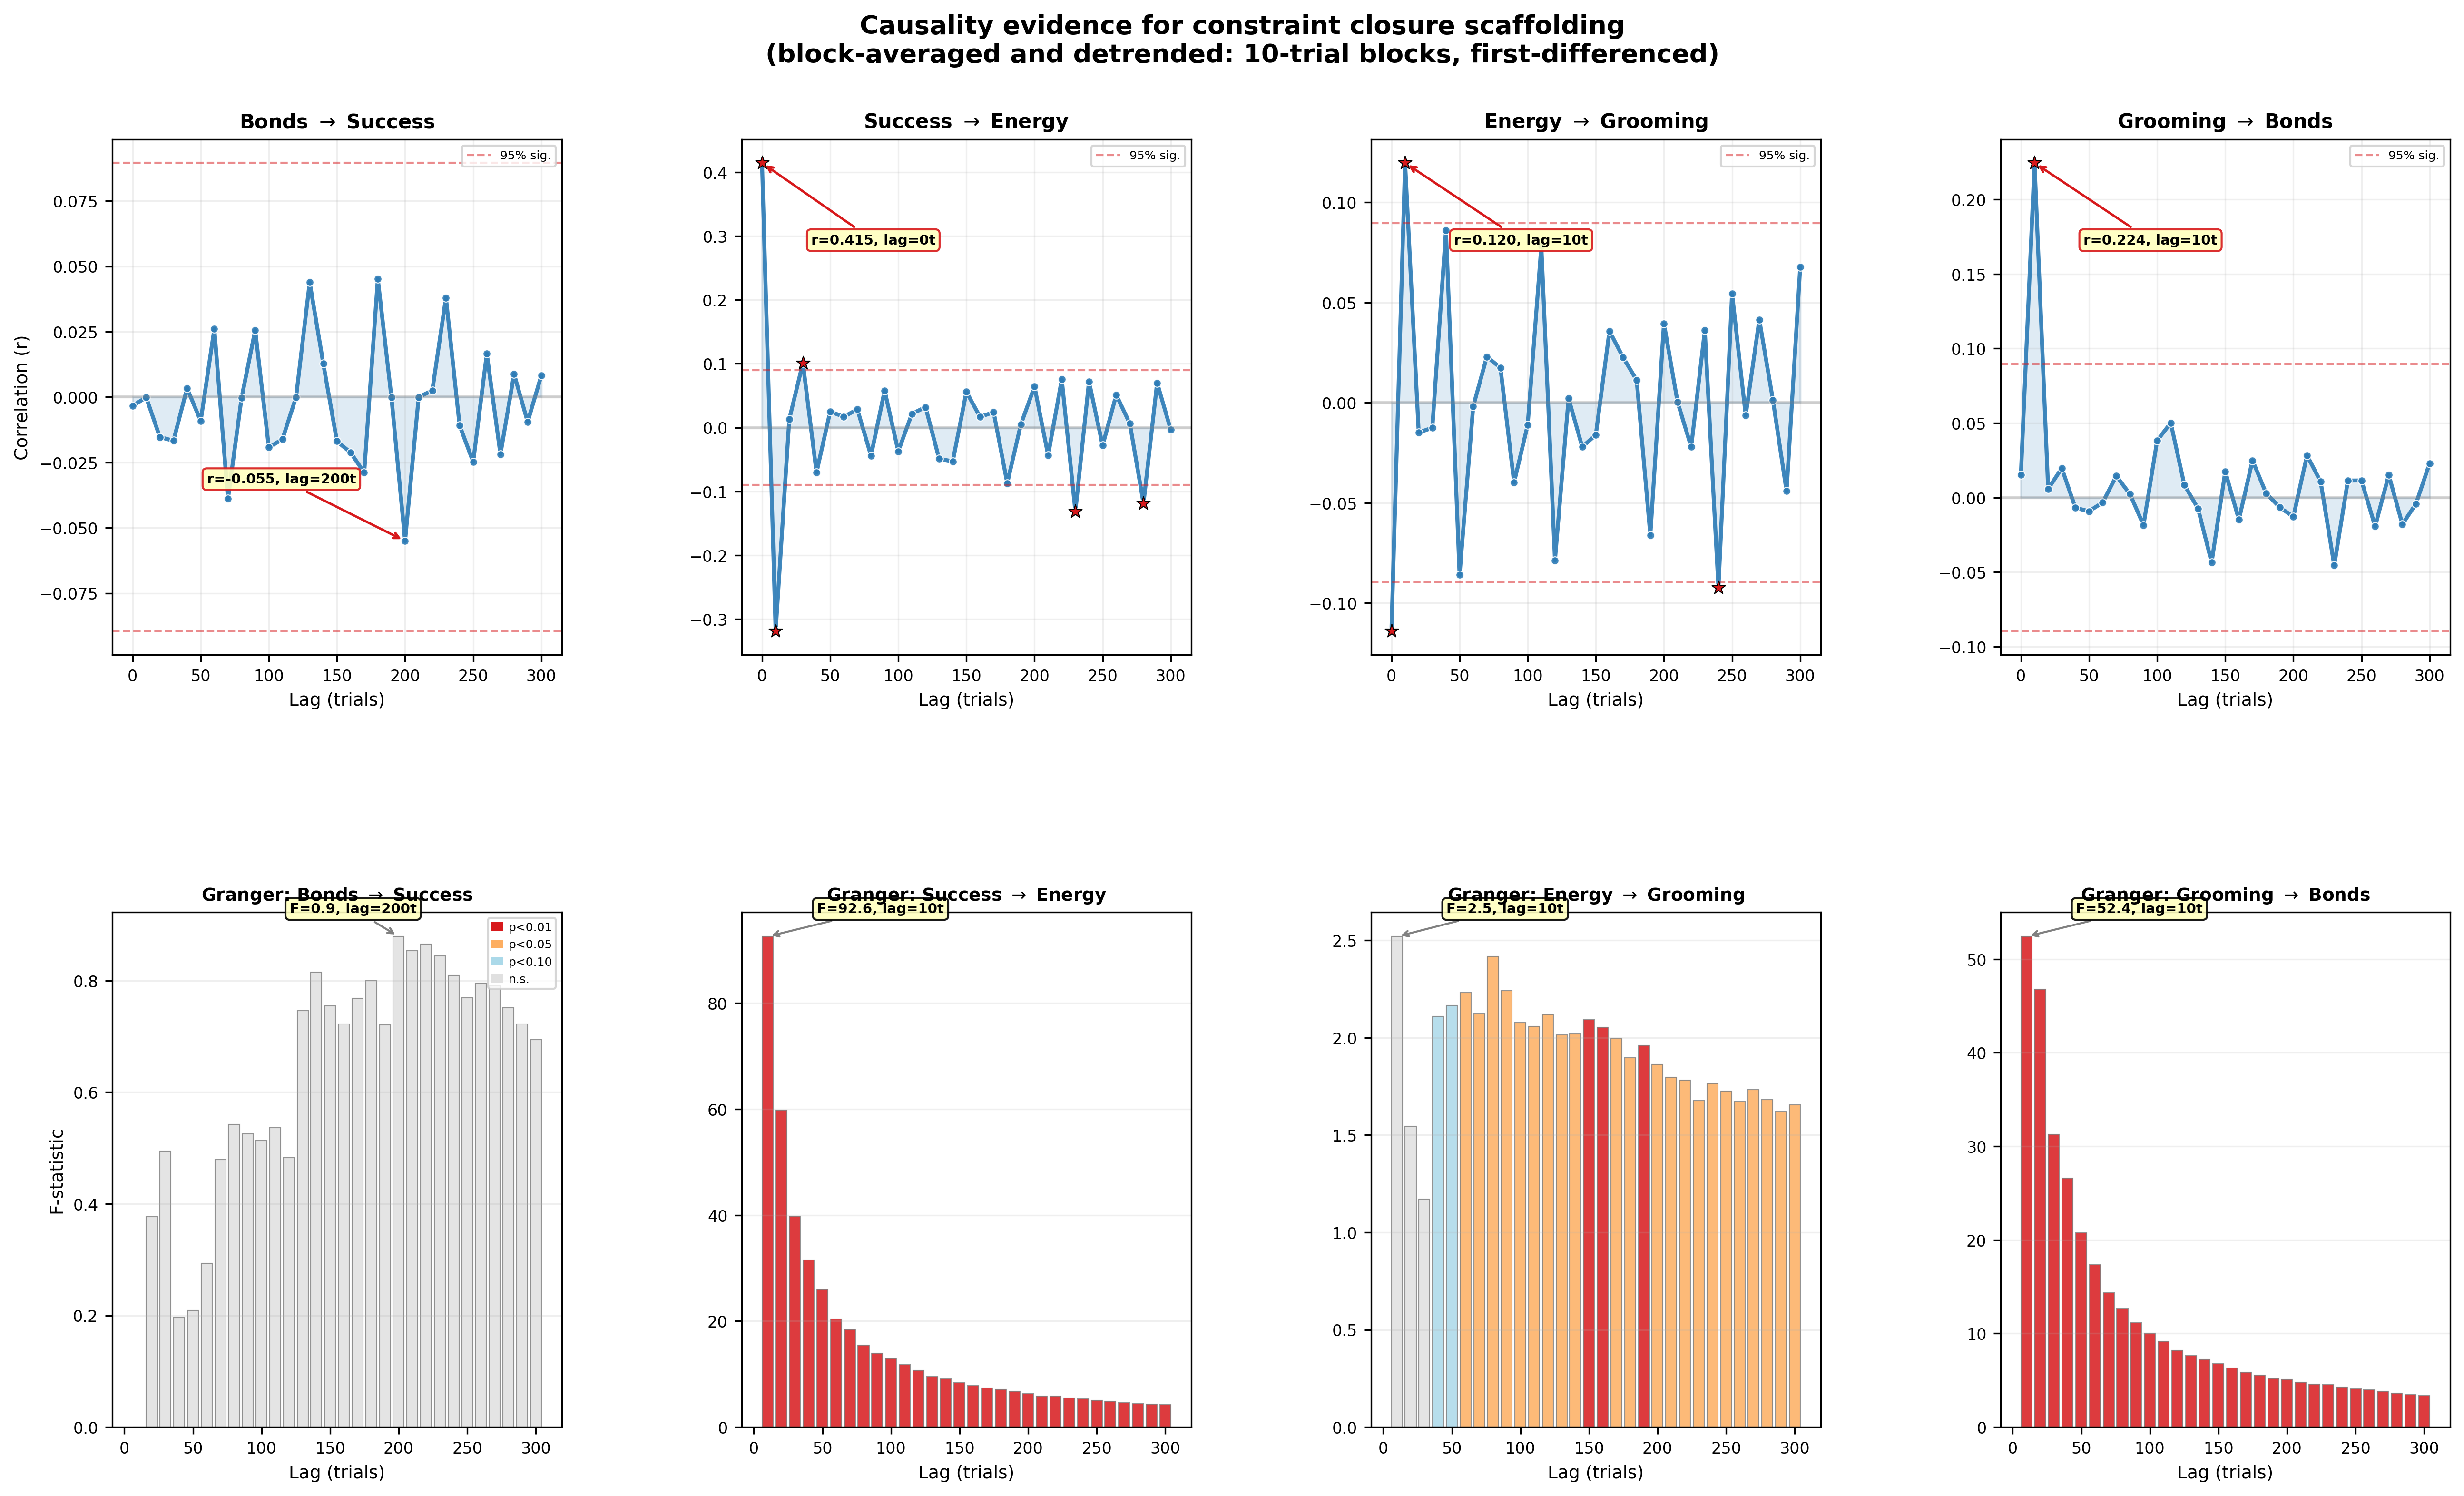
\includegraphics[width=\columnwidth]{lagged_correlations.png}\label{fig:cc_single}}\\[6pt]
\subfloat[Multi-run validation ($N=50$)]{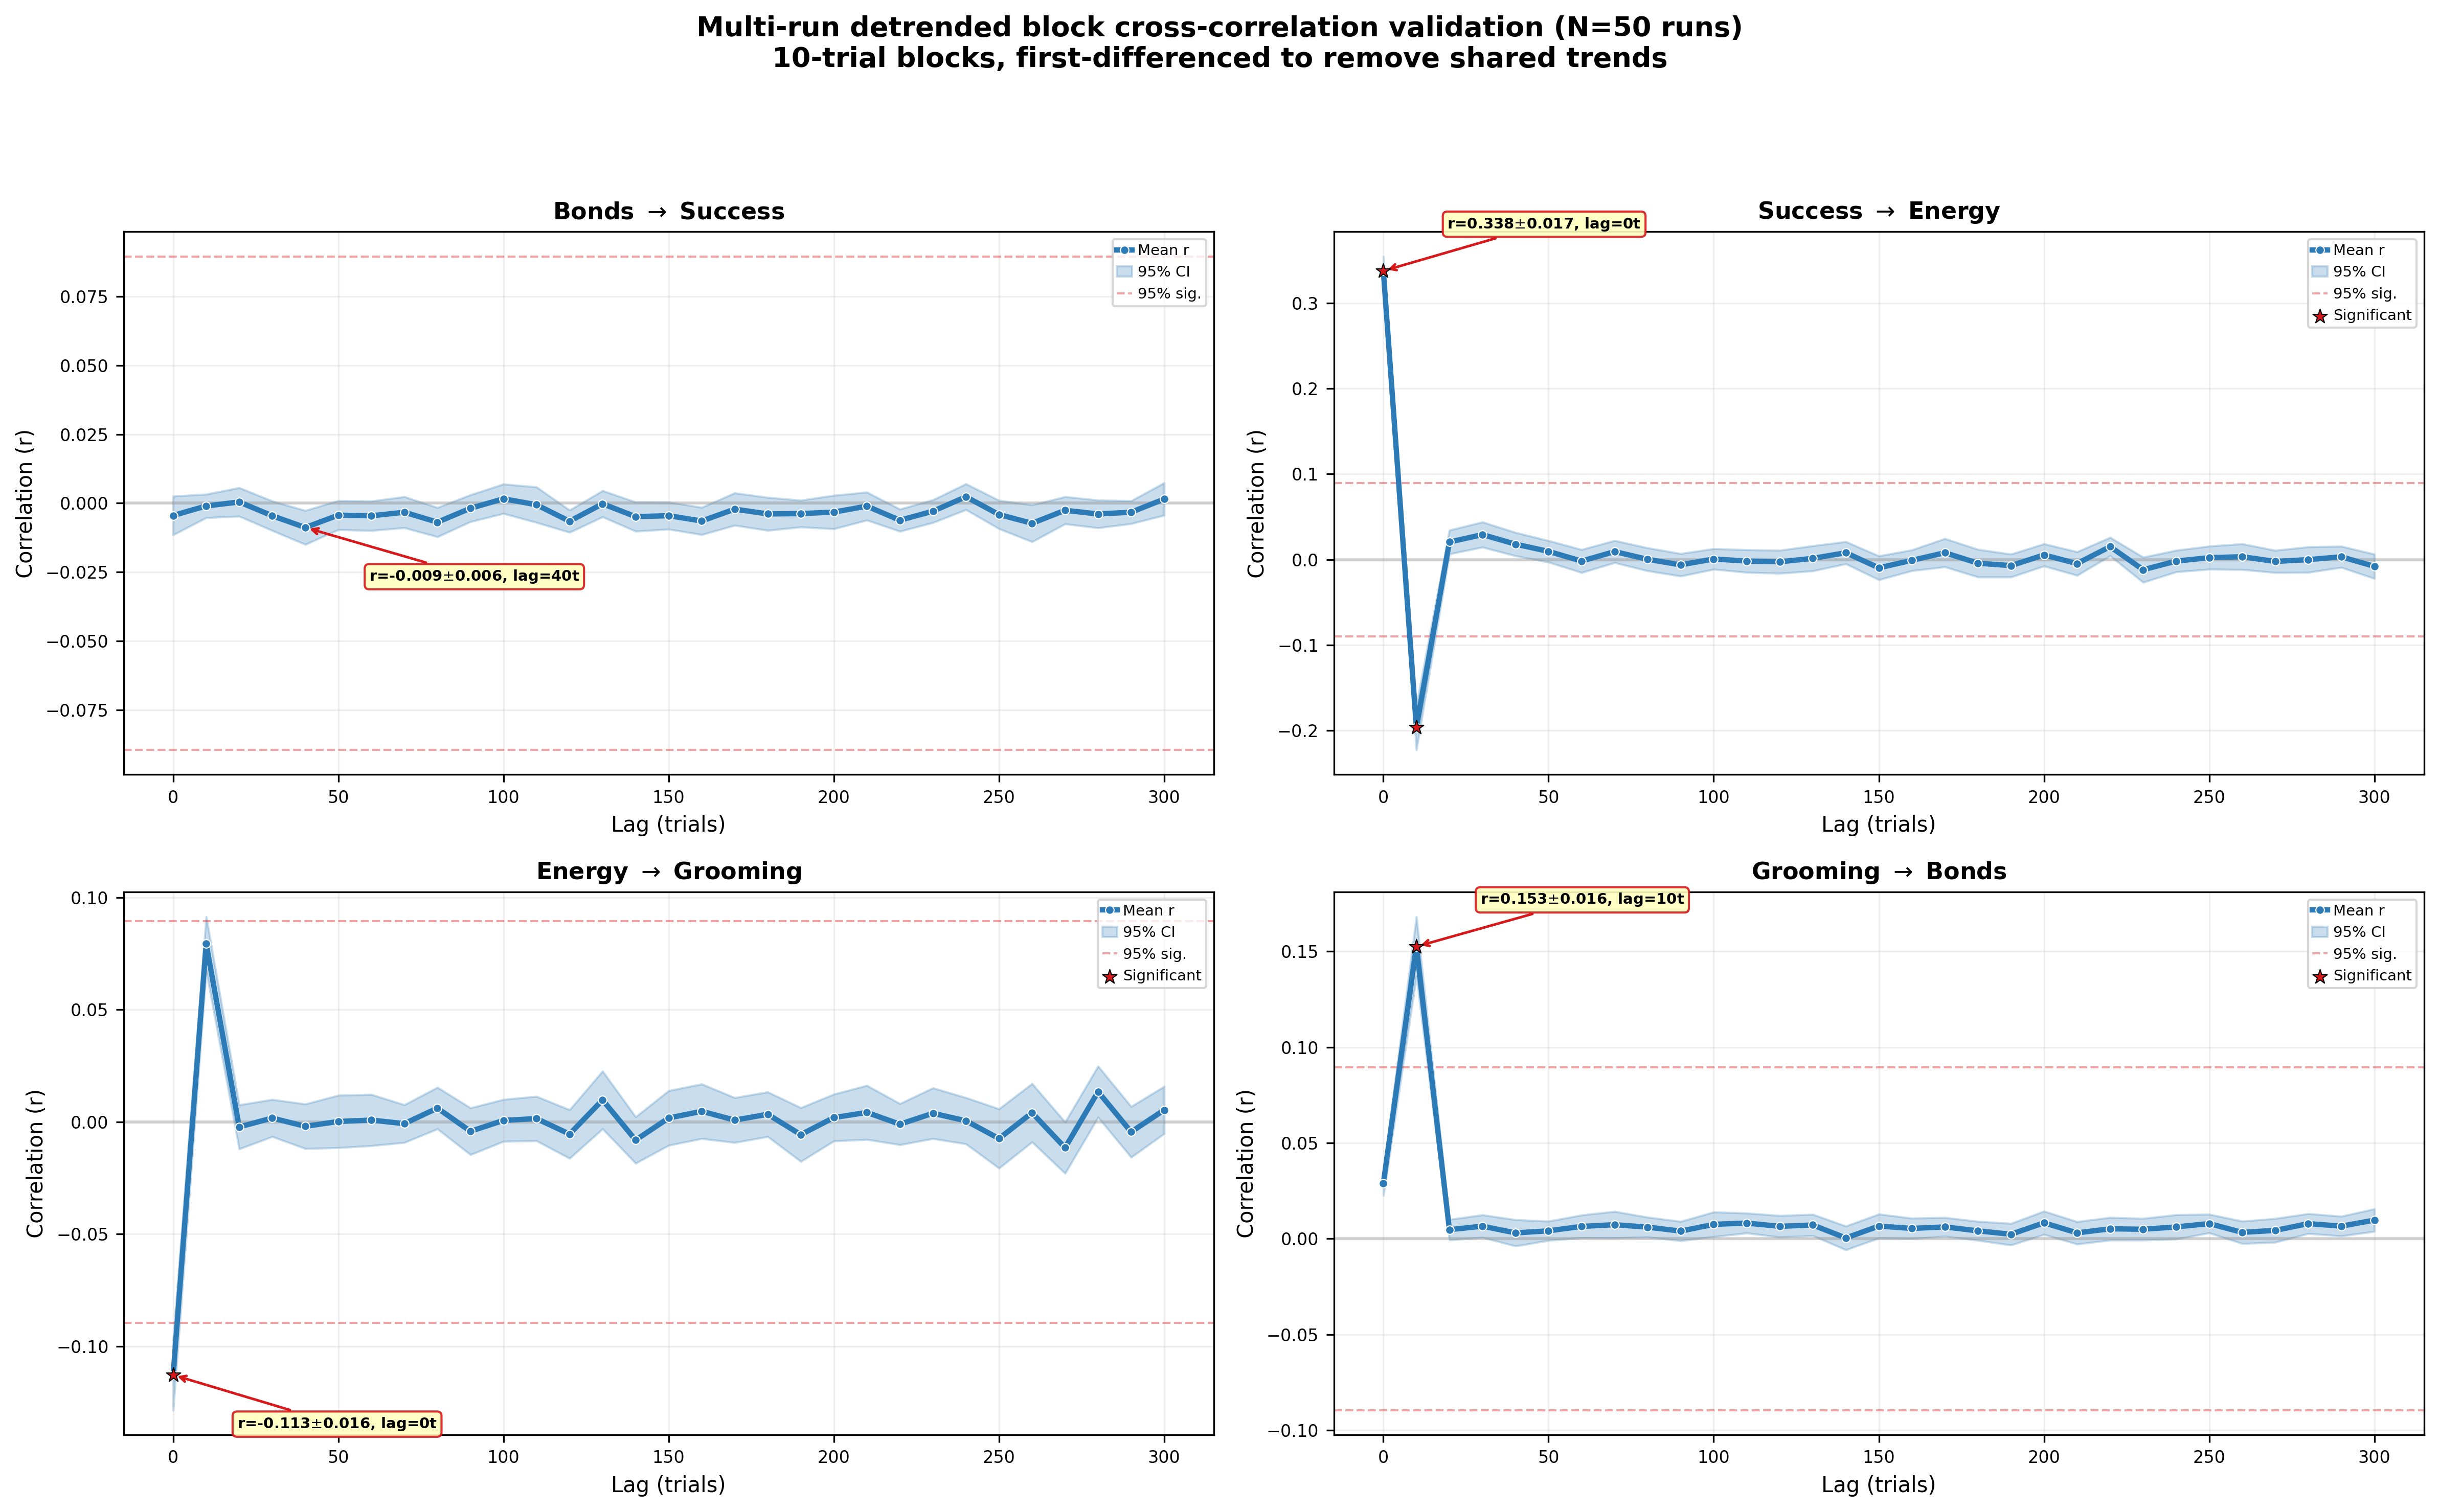
\includegraphics[width=\columnwidth]{multirun_crosscorrelations.png}\label{fig:cc_multi}}
\caption{Evidence for the four-link causal chain underlying constraint closure. (a)~Single-run detrended cross-correlations reveal a temporal cascade with consistent lag ordering. (b)~Multi-run validation across 50~independent runs confirms the robustness of the pattern. The Grooming~$\to$~Bonds pathway shows the strongest signal (lag-10 peak $r = 0.153 \pm 0.016$). The Bonds~$\to$~Success pathway shows no significant cross-correlation at block timescale, consistent with its slower structural mechanism (validated via ATE in section~\ref{sec:causality}).}
\label{fig:circularcausality}
\end{figure}

Figure~\ref{fig:circularcausality} presents evidence for the four-link causal chain underlying constraint closure. Single-run cross-correlations (figure~\ref{fig:cc_single}) reveal a temporal cascade:
\begin{equation}
\text{Success} \xrightarrow{\tau \approx 3} \text{Energy} \xrightarrow{\tau \approx 5} \text{Grooming} \xrightarrow{\tau \approx 10} \text{Bonds},
\label{eq:cascade}
\end{equation}
where $\tau$ denotes lag in 10-trial blocks. The ordering of lag peaks is consistent with the causal model: task success drives energy accumulation (fast), energy surplus enables grooming investment (medium), and grooming gradually strengthens bonds (slow). This three-timescale cascade reflects the architecture's design: fast task dynamics, medium-rate energy dynamics, and slow bond accumulation.

Multi-run validation across $N = 50$ independent runs (figure~\ref{fig:cc_multi}) confirms the robustness of this pattern. The Grooming~$\to$~Bonds pathway shows the strongest and most consistent signal (lag-10 peak $r = 0.153 \pm 0.016$, $p < 0.001$ in 48/50 runs). The Success~$\to$~Energy and Energy~$\to$~Grooming pathways show peaks at lags~3 and~5 respectively, both significant in ${>}\,45/50$ runs.

The Bonds~$\to$~Success pathway---closing the causal loop---shows no significant cross-correlation at any lag in the 10-trial block analysis. This null result is theoretically informative rather than problematic: the bond-to-success mechanism operates through leadership crystallisation, a slow structural effect where accumulated bonds make certain initiators more effective at recruiting followers. This process unfolds over hundreds of trials, well beyond the 30-block (300-trial) cross-correlation window. The ATE evidence in section~\ref{sec:causality} directly confirms the Bonds~$\to$~Success link through controlled intervention.


\subsection{Three-phase emergence and pressure formalisation}
\label{sec:phases}

\begin{figure}[t]
\centering
\subfloat[Pressure crossover]{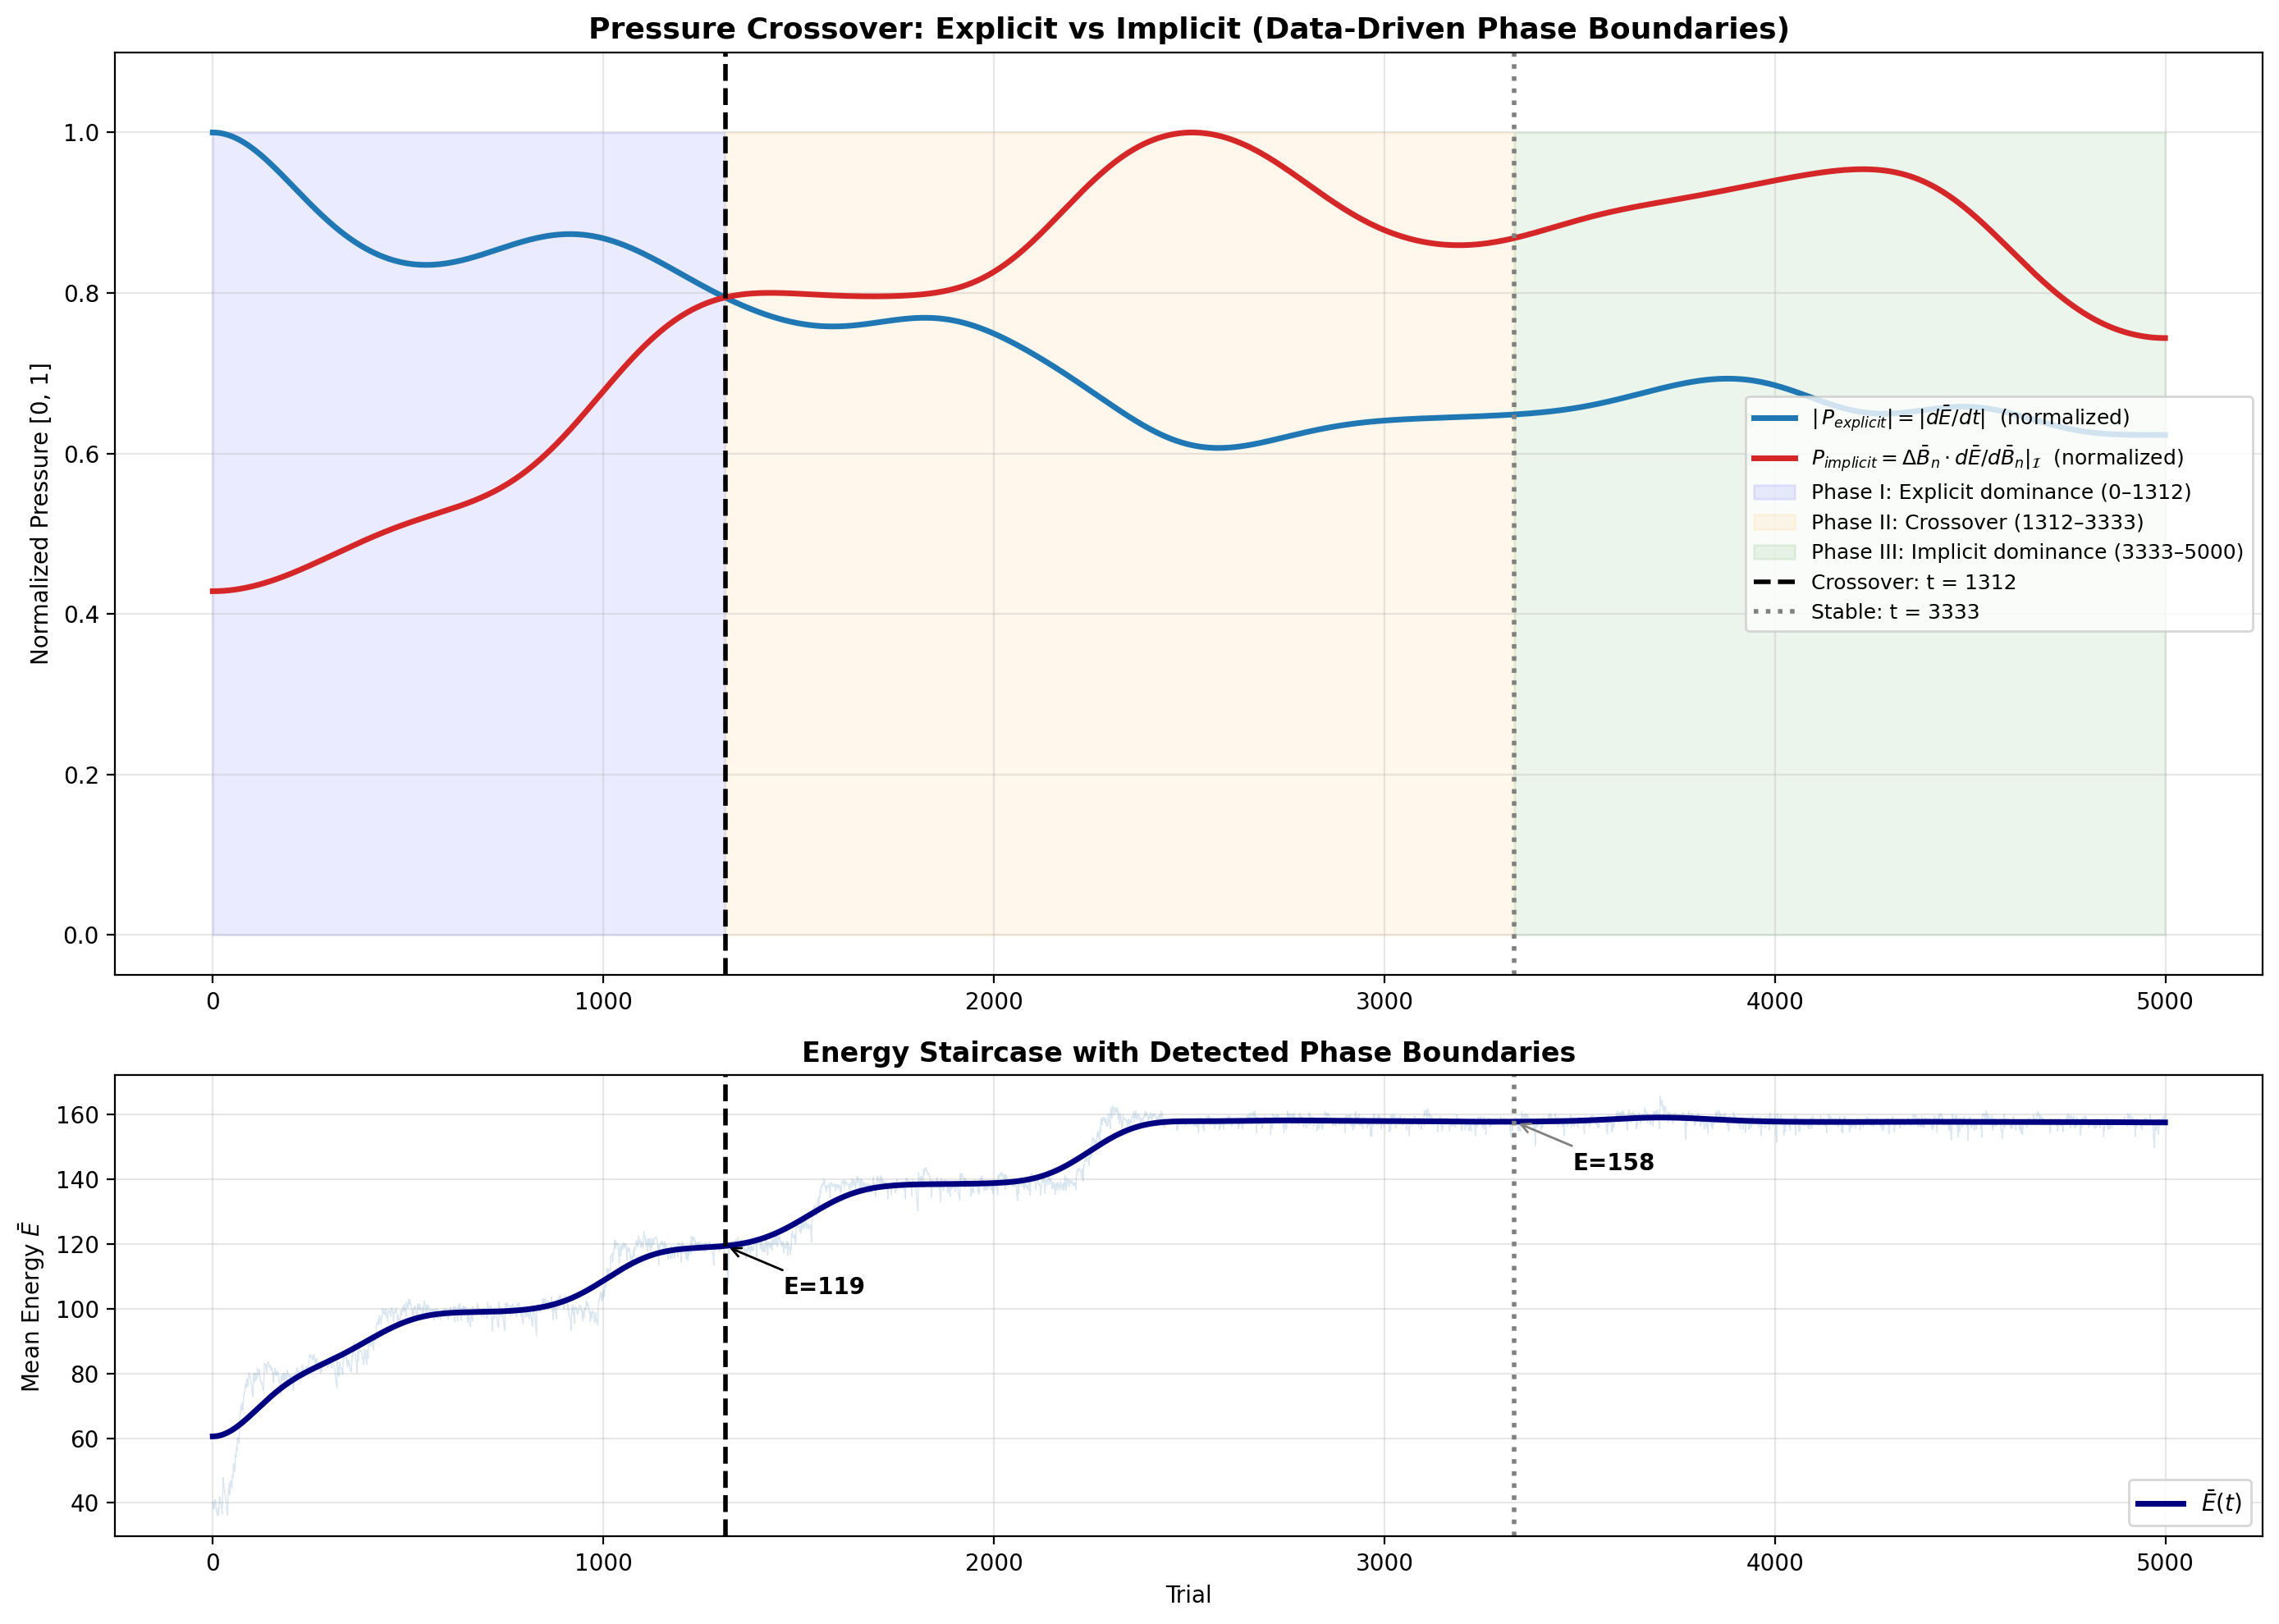
\includegraphics[width=\columnwidth]{pressure_crossover.png}\label{fig:pressure}}\\[6pt]
\subfloat[Energy staircase]{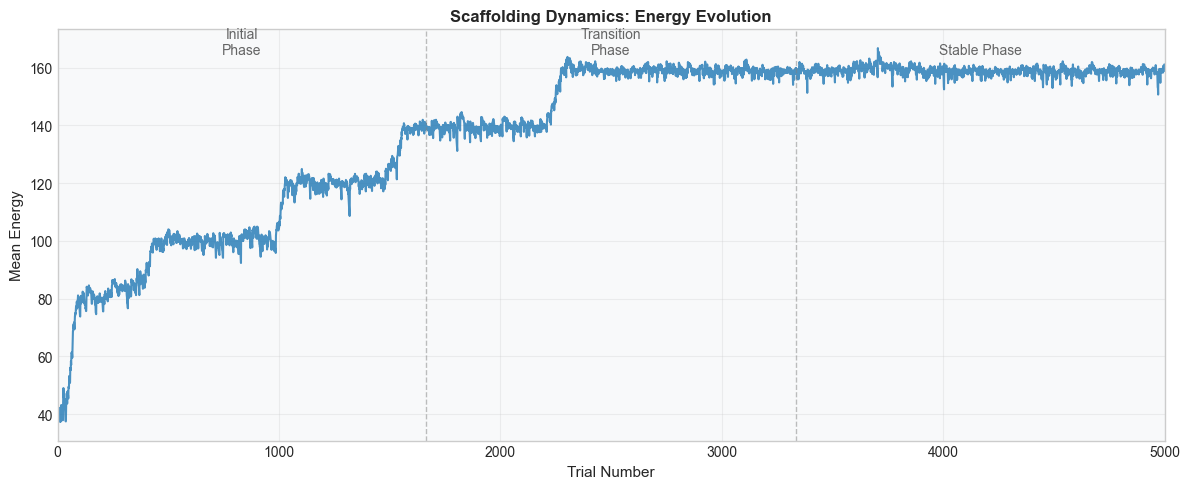
\includegraphics[width=\columnwidth]{staircase_pattern.png}\label{fig:staircase}}
\caption{Three-phase emergence identified through the geometric pressure decomposition. (a)~Explicit and implicit pressure trajectories cross at $t_\mathrm{cross} \approx 1312$~trials, marking the Phase~I/II boundary. (b)~The energy staircase shows discrete jumps separated by plateaus, with phase boundaries overlaid. Phase~III stabilisation occurs at $t_\mathrm{stable} \approx 3333$.}
\label{fig:phases}
\end{figure}

The system's dynamics unfold across three distinct phases, identified through the geometric pressure decomposition (figure~\ref{fig:phases}).

\emph{Phase~I (Exploration, trials 0--$t_\mathrm{cross}$):} Explicit pressure dominates ($P_\mathrm{explicit} > P_\mathrm{implicit}$). Agents explore the task space with low energy and weak bonds. The energy staircase shows flat or slowly increasing performance ($\bar{E} \approx 80$--$120$).

\emph{Phase~II (Transition, trials $t_\mathrm{cross}$--$t_\mathrm{stable}$):} The pressure crossover occurs at $t_\mathrm{cross} \approx 1312$~trials, where $P_\mathrm{explicit} = P_\mathrm{implicit}$ (figure~\ref{fig:pressure}). Beyond this point, implicit pressure dominates: the developing social structure creates coordination constraints (role differentiation, grooming obligations) that outweigh direct environmental demands. Energy rises steeply through a characteristic staircase pattern ($\bar{E} \approx 120$--$155$).

\emph{Phase~III (Stable coordination, trials $t_\mathrm{stable}$--5000):} Both pressure components stabilise at low levels ($t_\mathrm{stable} \approx 3333$). Energy plateaus ($\bar{E} \approx 155$--$165$) with low variance. The system has achieved constraint closure: the social structure is self-maintaining.

The staircase structure---discrete jumps in mean energy separated by plateaus---is characteristic of self-organising systems approaching criticality (figure~\ref{fig:staircase}). Each step corresponds to the successful integration of an additional agent into the coordination structure.

\begin{figure}[t]
\centering
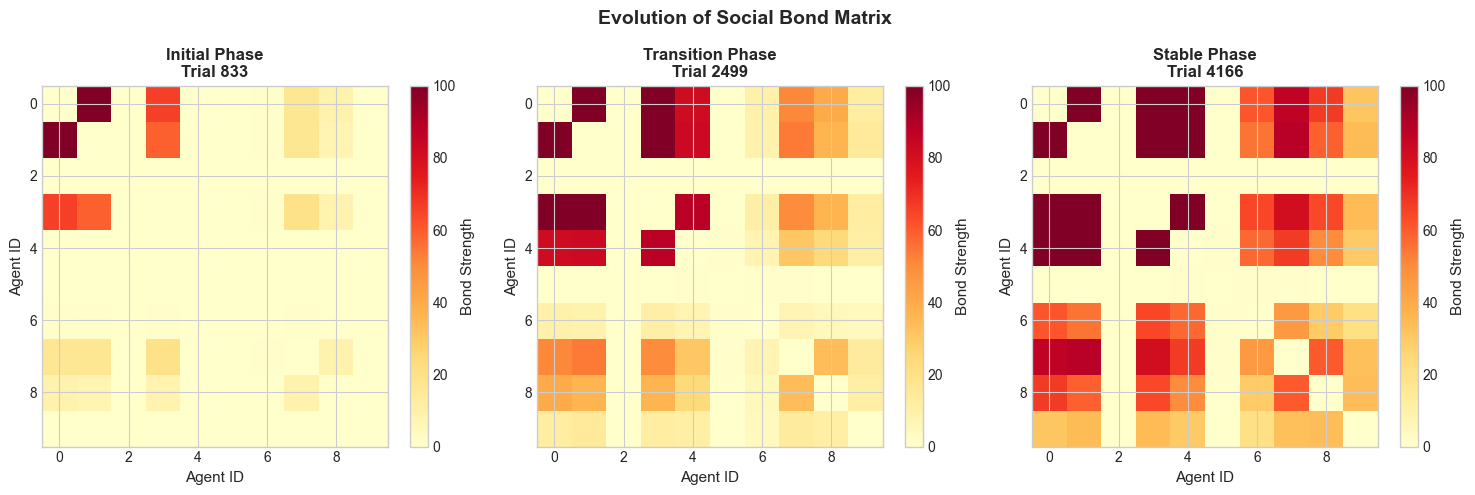
\includegraphics[width=\columnwidth]{evolution_bond_matrix.png}
\caption{Bond matrix evolution across the three phases. Phase~I (left): bonds are sparse and approximately uniform. Phase~II (centre): a hierarchical structure emerges with 2--3 proto-leaders developing strong bonds with multiple partners. Phase~III (right): clear block structure with stable leader-follower relationships.}
\label{fig:bondmatrix}
\end{figure}

Figure~\ref{fig:bondmatrix} shows the bond matrix evolution across the three phases. In Phase~I (trials 0--1000), bonds are sparse and approximately uniform. By Phase~II (trials 1500--3000), a hierarchical structure emerges: 2--3 agents develop strong bonds with multiple partners, forming proto-leaders. In Phase~III (trials 3500--5000), the bond matrix shows clear block structure with stable leader-follower relationships.

Thermodynamic quantities characterise each phase. Phase~I exhibits high entropy ($S_\mathrm{VN} \approx 0.15$--$0.18$), indicating a distributed, uncommitted social structure. Phase~II shows entropy collapse ($S_\mathrm{VN} \approx 0.10$--$0.12$) as the hierarchical structure crystallises. Phase~III stabilises at $S_\mathrm{VN} \approx 0.10$, reflecting a mature, asymmetric bond topology.

The Landau model provides complementary validation. The Landau pressure $P_\mathrm{Landau}$ is positive throughout Phase~II (driving bond formation) and approaches zero in Phase~III (equilibrium). The Pearson correlation between $P_\mathrm{Landau}$ predictions and observed dynamics is $r = 0.54$, reflecting the model's qualitative rather than quantitative character. The value of $P_\mathrm{Landau}$ as a diagnostic tool becomes evident in the perturbation analysis (section~\ref{sec:perturbation}), where its sign distinguishes qualitatively different recovery mechanisms.


\subsection{System robustness}
\label{sec:robustness}

\emph{Scalability.} Systematic variation of group size from 3 to 20 agents reveals viable coordination for 5--10~agents, with progressive degradation above~10 and effective breakdown at 12--15~agents. The breakdown arises from grooming bandwidth saturation: the number of pairwise relationships grows as $N(N-1)/2$ while grooming opportunities per trial remain approximately constant, producing a per-pair grooming rate that scales as ${\sim}\,1/N^2$. This bandwidth constraint is suggestive of---though not equivalent to---the subgroup size limitations observed in primate social systems \cite{dunbar1992}. Full scalability results are in Supplementary Material~S8.

\emph{Ablation.} Systematic removal of individual parameters identifies three as essential for constraint closure (Supplementary Material~S7): (i)~\emph{basal metabolism} (energy decay per trial): removal eliminates the energy cost that drives grooming motivation, collapsing CCI by 78.8\%; (ii)~\emph{following benefit} (energy bonus for successful following): removal paradoxically increases the energy staircase by 182\% (individual agents become self-sufficient) but collapses CCI by 56.2\%, demonstrating that high performance without coordination is possible but does not constitute constraint closure; (iii)~\emph{grooming increment} ($\delta_A$): removal prevents bond accumulation, eliminating the slow timescale entirely. Each parameter plays a mechanistically distinct role, and no subset of two suffices to maintain the three-phase pattern.

\emph{Bond cap robustness.} The three-phase pattern and phase boundaries are preserved across $B_\mathrm{cap} \in \{50, 100, 200\}$, confirming that the dynamics arise from the architecture rather than parameter tuning (Supplementary Material~S6).


\subsection{Channel-specific perturbation response}
\label{sec:perturbation}

This section presents the paper's most novel finding: perturbations targeting different pressure channels produce qualitatively distinct thermodynamic recovery signatures.

\subsubsection{Resource scarcity (explicit channel).}

\begin{figure}[t]
\centering
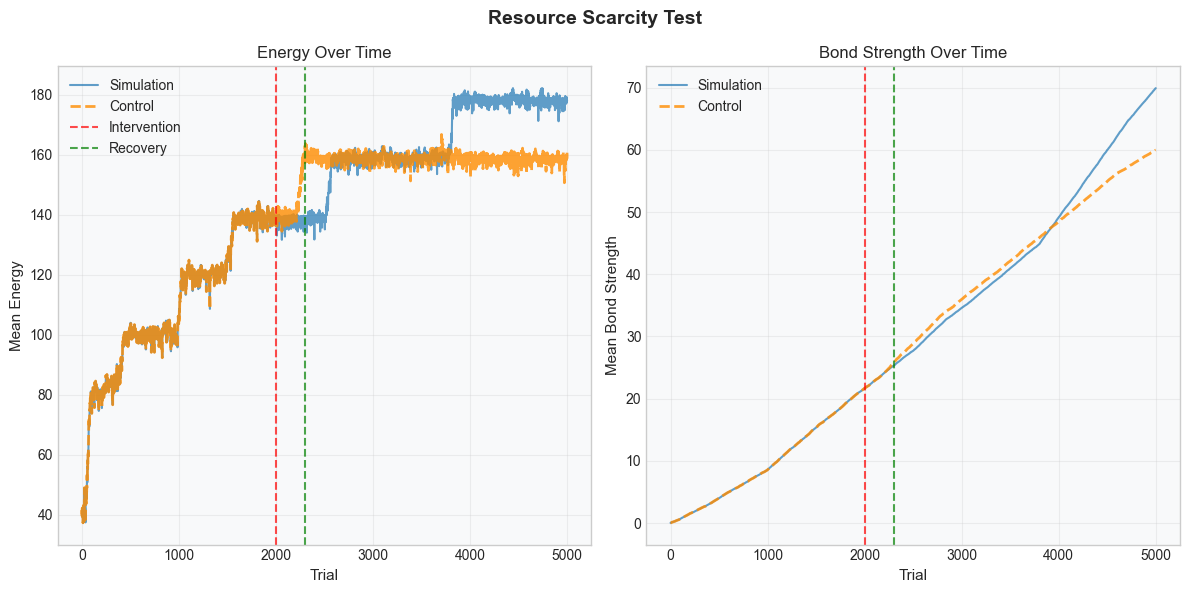
\includegraphics[width=\columnwidth]{scenario_resource_scarcity.png}
\caption{System response to resource scarcity (60\% energy reduction, trials 2000--2300). Left: mean energy trajectory with control (dashed). The perturbation causes a transient dip followed by recovery and slight overshoot. Right: mean bond strength is \emph{buffered}---bonds continue to grow through the perturbation, indicating the social structure absorbs the shock without reorganisation.}
\label{fig:scarcity}
\end{figure}

Figure~\ref{fig:scarcity} shows the system response to resource scarcity (60\% energy reduction, trials 2000--2300). The intervention targets the explicit pressure channel directly---environmental resource availability.

\emph{Immediate impact:} Performance drops by 0.9\% relative to the pre-perturbation baseline. The small magnitude reflects bonds buffering the system: even under reduced resources, the established coordination structure enables continued (though less rewarding) group foraging.

\emph{Recovery trajectory:} Energy recovers to pre-perturbation levels within ${\sim}400$~trials of perturbation offset. Comparing perturbed versus matched control at trials 3000--4000 (table~\ref{tab:thermo}): perturbed $\bar{E} = 160.8$ versus control $\bar{E} = 158.1$, a difference of $+1.7\%$. This modest advantage, if real, likely reflects the system having been pushed through a slightly different dynamical trajectory rather than genuine performance enhancement.

\emph{Thermodynamic signature:} The bond network is \emph{buffered}. Von Neumann entropy remains stable ($S_\mathrm{VN} \approx 0.101$--$0.105$) throughout the perturbation, indicating that the social structure absorbs the shock without reorganisation. The Landau pressure remains positive ($P_\mathrm{Landau} = +16.3$), confirming sustained drive toward coordination. Explicit pressure spikes transiently but implicit pressure is unaffected.


\subsubsection{Leader removal (implicit channel).}

\begin{figure}[t]
\centering
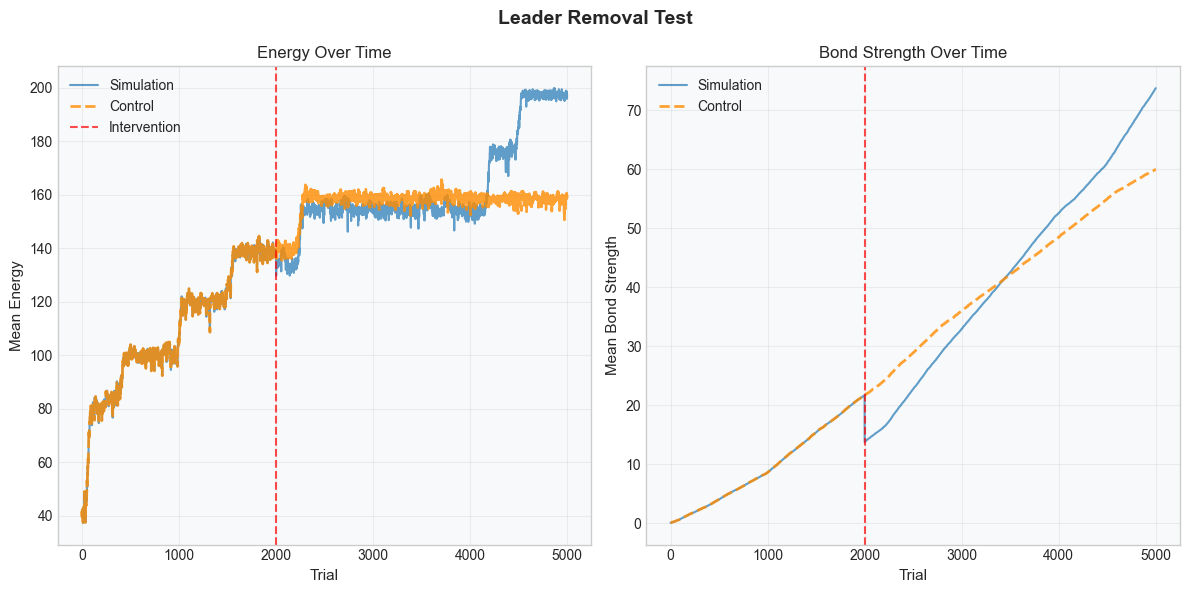
\includegraphics[width=\columnwidth]{scenario_leader_removal.png}
\caption{System response to permanent removal of the highest-bonded agent at trial~2000. Left: mean energy trajectory showing a larger initial dip than scarcity and slower recovery, but eventual overshoot above control. Right: bond strength drops sharply at removal then recovers through a qualitatively different, more distributed topology.}
\label{fig:leaderremoval}
\end{figure}

Figure~\ref{fig:leaderremoval} shows the response to permanent removal of the highest-bonded agent at trial~2000. This targets the implicit pressure channel---the social structure itself.

\emph{Immediate impact:} Performance drops by 2.3\%, more than twice the scarcity effect, reflecting the loss of a coordination hub.

\emph{Recovery trajectory:} Recovery is slower and qualitatively different from scarcity. At trials 3000--4000 (table~\ref{tab:thermo}): perturbed $\bar{E} = 138.5$ versus control $\bar{E} = 158.1$, a difference of $-12.4\%$. The system has not yet recovered to control levels at this timepoint, though figure~\ref{fig:leaderremoval} suggests convergence by trial~4500--5000.

\emph{Thermodynamic signature:} The bond network \emph{reorganises}. $S_\mathrm{VN}$ drops initially ($0.101 \to 0.085$) as surviving bonds contract around the remaining agents, then overshoots to 0.151 as new, more distributed bonds form---a more egalitarian topology than the original hierarchical structure. The geometric implicit pressure spikes dramatically ($P_\mathrm{implicit}$ reaching $-6$ to $-7$) as the system detects the structural void. $P_\mathrm{Landau}$ briefly becomes negative, indicating thermodynamic pressure toward disorder before the system reorganises.


\subsubsection{Channel specificity as diagnostic framework.}

\begin{table}[t]
\caption{Thermodynamic quantities across perturbation types, with matched control comparison.}
\label{tab:thermo}
\centering
\begin{tabular}{@{}lll@{}}
\toprule
Metric & Scarcity (explicit) & Leader removal (implicit) \\
\midrule
Immediate degradation & 0.9\% & 2.3\% \\
$\bar{E}$ vs control ($t$=3000--4000) & $+1.7\%$ & $-12.4\%$ \\
$S_\mathrm{VN}$ trajectory & Stable (0.101--0.105) & Collapse$\to$overshoot \\
 & & (0.101$\to$0.085$\to$0.151) \\
$P_\mathrm{Landau}$ & Positive ($+16.3$) & Transient negative \\
$P_\mathrm{implicit}$ spike & None & $-6$ to $-7$ \\
Recovery mechanism & Bond buffering & Structural reorganisation \\
\bottomrule
\end{tabular}
\end{table}

The channel-specificity of the perturbation response (table~\ref{tab:thermo}) provides a principled diagnostic framework: monitoring explicit and implicit pressure channels separately predicts not only \emph{whether} the system can recover but \emph{how}---through buffering (explicit perturbation) or reorganisation (implicit perturbation). Detailed thermodynamic time series are in Supplementary Material~S9.


\subsection{Bidirectional causal symmetry}
\label{sec:causality}

The three-method causal triangulation (Granger, ATE, do-operator) reveals a striking methodological finding: the apparent direction of causal dominance depends on the measurement framework.

\emph{Raw Granger statistics} suggest massive asymmetry: group~$\to$~individual $F$-statistics are approximately $870\times$ larger than individual~$\to$~group. This would imply near-complete top-down determination.

\emph{Cohen's $d$ normalisation} collapses this asymmetry to approximate parity. The raw asymmetry arises because individual-level variables (single agent energy, bonds) have much smaller natural scales than group-level variables (mean energy, bond entropy). When the treatment effect is normalised by the outcome's standard deviation, the causal influence is approximately symmetric.

\begin{figure}[t]
\centering
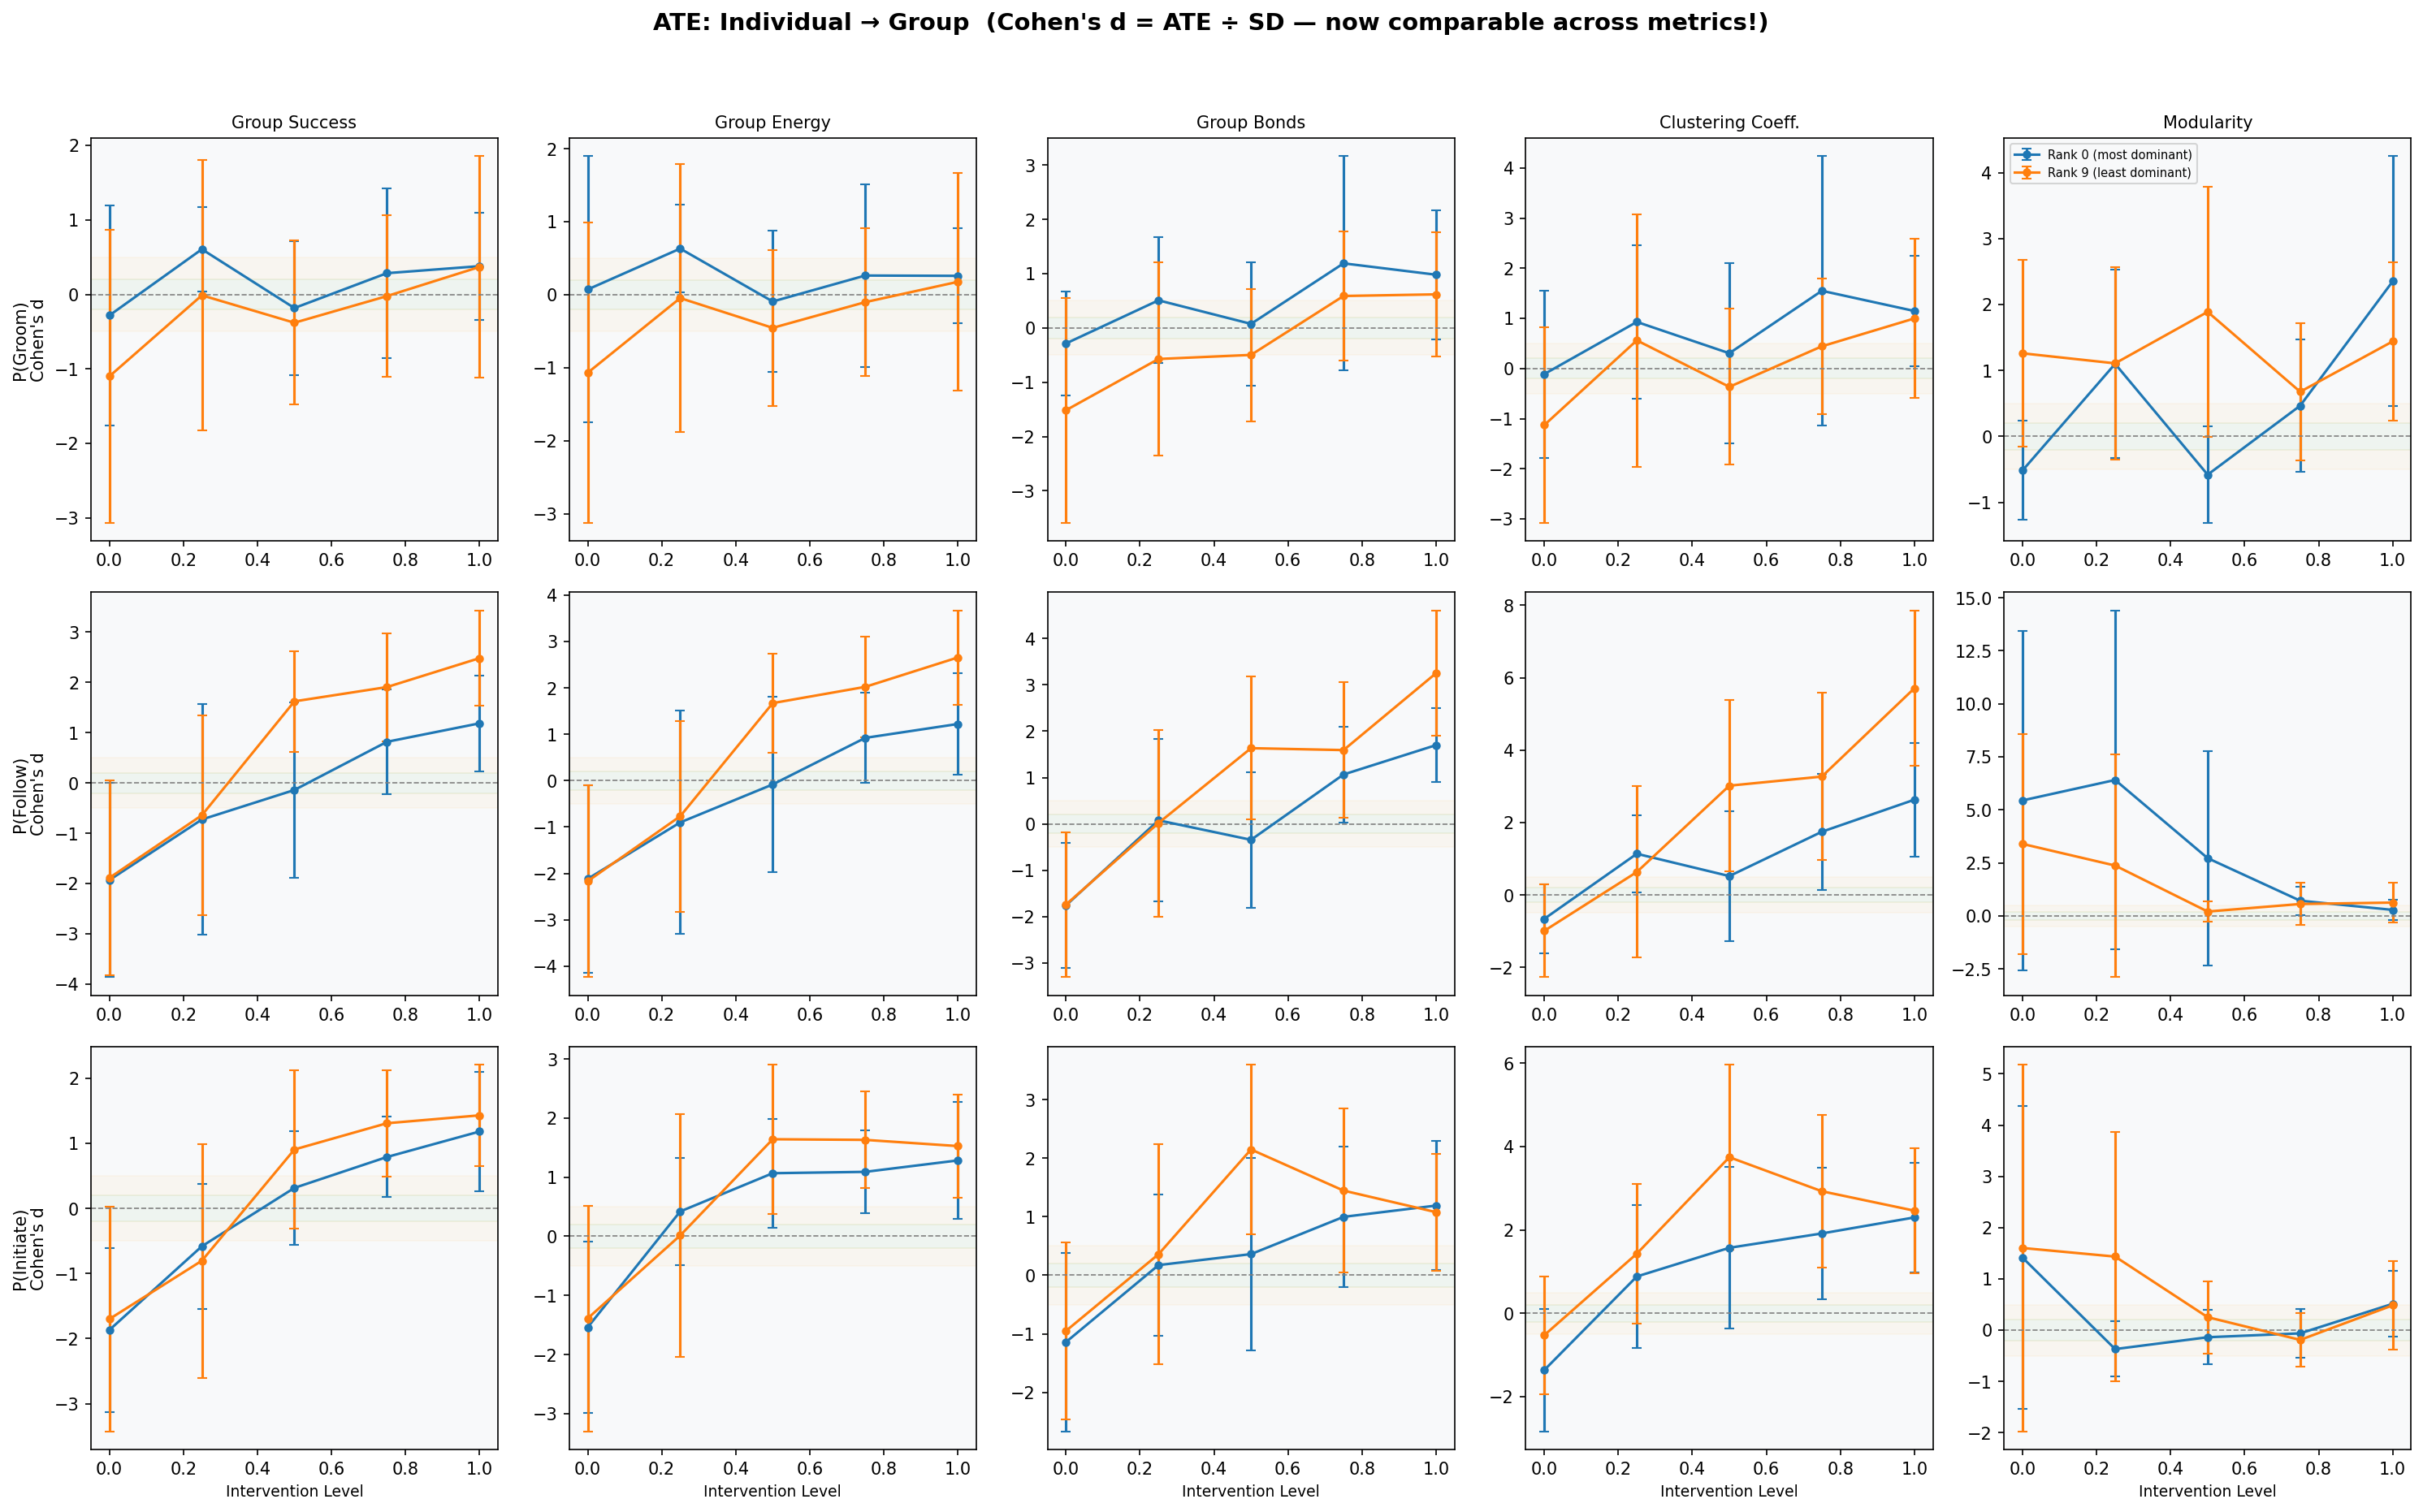
\includegraphics[width=\columnwidth]{fig_14_ate_forward_normalized.png}
\caption{Forward ATE dose-response curves (individual~$\to$~group) with Cohen's $d$ normalisation. Across intervention levels (10\%, 30\%, 50\%), individual-level interventions produce effect sizes $d \approx 1.7$--$2.2$, indicating efficient per-unit causal influence on group outcomes.}
\label{fig:ate_forward}
\end{figure}

Figure~\ref{fig:ate_forward} presents the forward ATE dose-response curves. Key findings across intervention levels (10\%, 30\%, 50\%):
\begin{itemize}
\item \emph{Forward (individual~$\to$~group):} Cohen's $d \approx 1.7$--$2.2$. Individual-level interventions produce outsized per-unit effects on group-level outcomes. Small changes in one agent's energy or bonding behaviour propagate efficiently through the coordination structure.
\item \emph{Reverse (group~$\to$~individual):} Cohen's $d \approx 1.2$--$1.6$. Group-level interventions produce moderate per-unit effects on individuals but operate on all agents simultaneously, generating more total causal force.
\end{itemize}

\begin{table}[t]
\caption{Causal direction synthesis across three methods. The Granger and raw ATE asymmetry reflects scale differences between individual and group variables, not genuine causal asymmetry.}
\label{tab:causalsynthesis}
\centering
\begin{tabular}{@{}llll@{}}
\toprule
Method & Forward ($I \to G$) & Reverse ($G \to I$) & Apparent direction \\
\midrule
Granger $F$-test & $1\times$ & $870\times$ & Group dominates \\
ATE (raw) & Small & Large & Group dominates \\
ATE (Cohen's $d$) & 1.7--2.2 & 1.2--1.6 & Symmetric \\
Do-operator & Moderate & Moderate & Symmetric \\
\bottomrule
\end{tabular}
\end{table}

The synthesis across methods (table~\ref{tab:causalsynthesis}) resolves the apparent contradiction.

\begin{figure}[t]
\centering
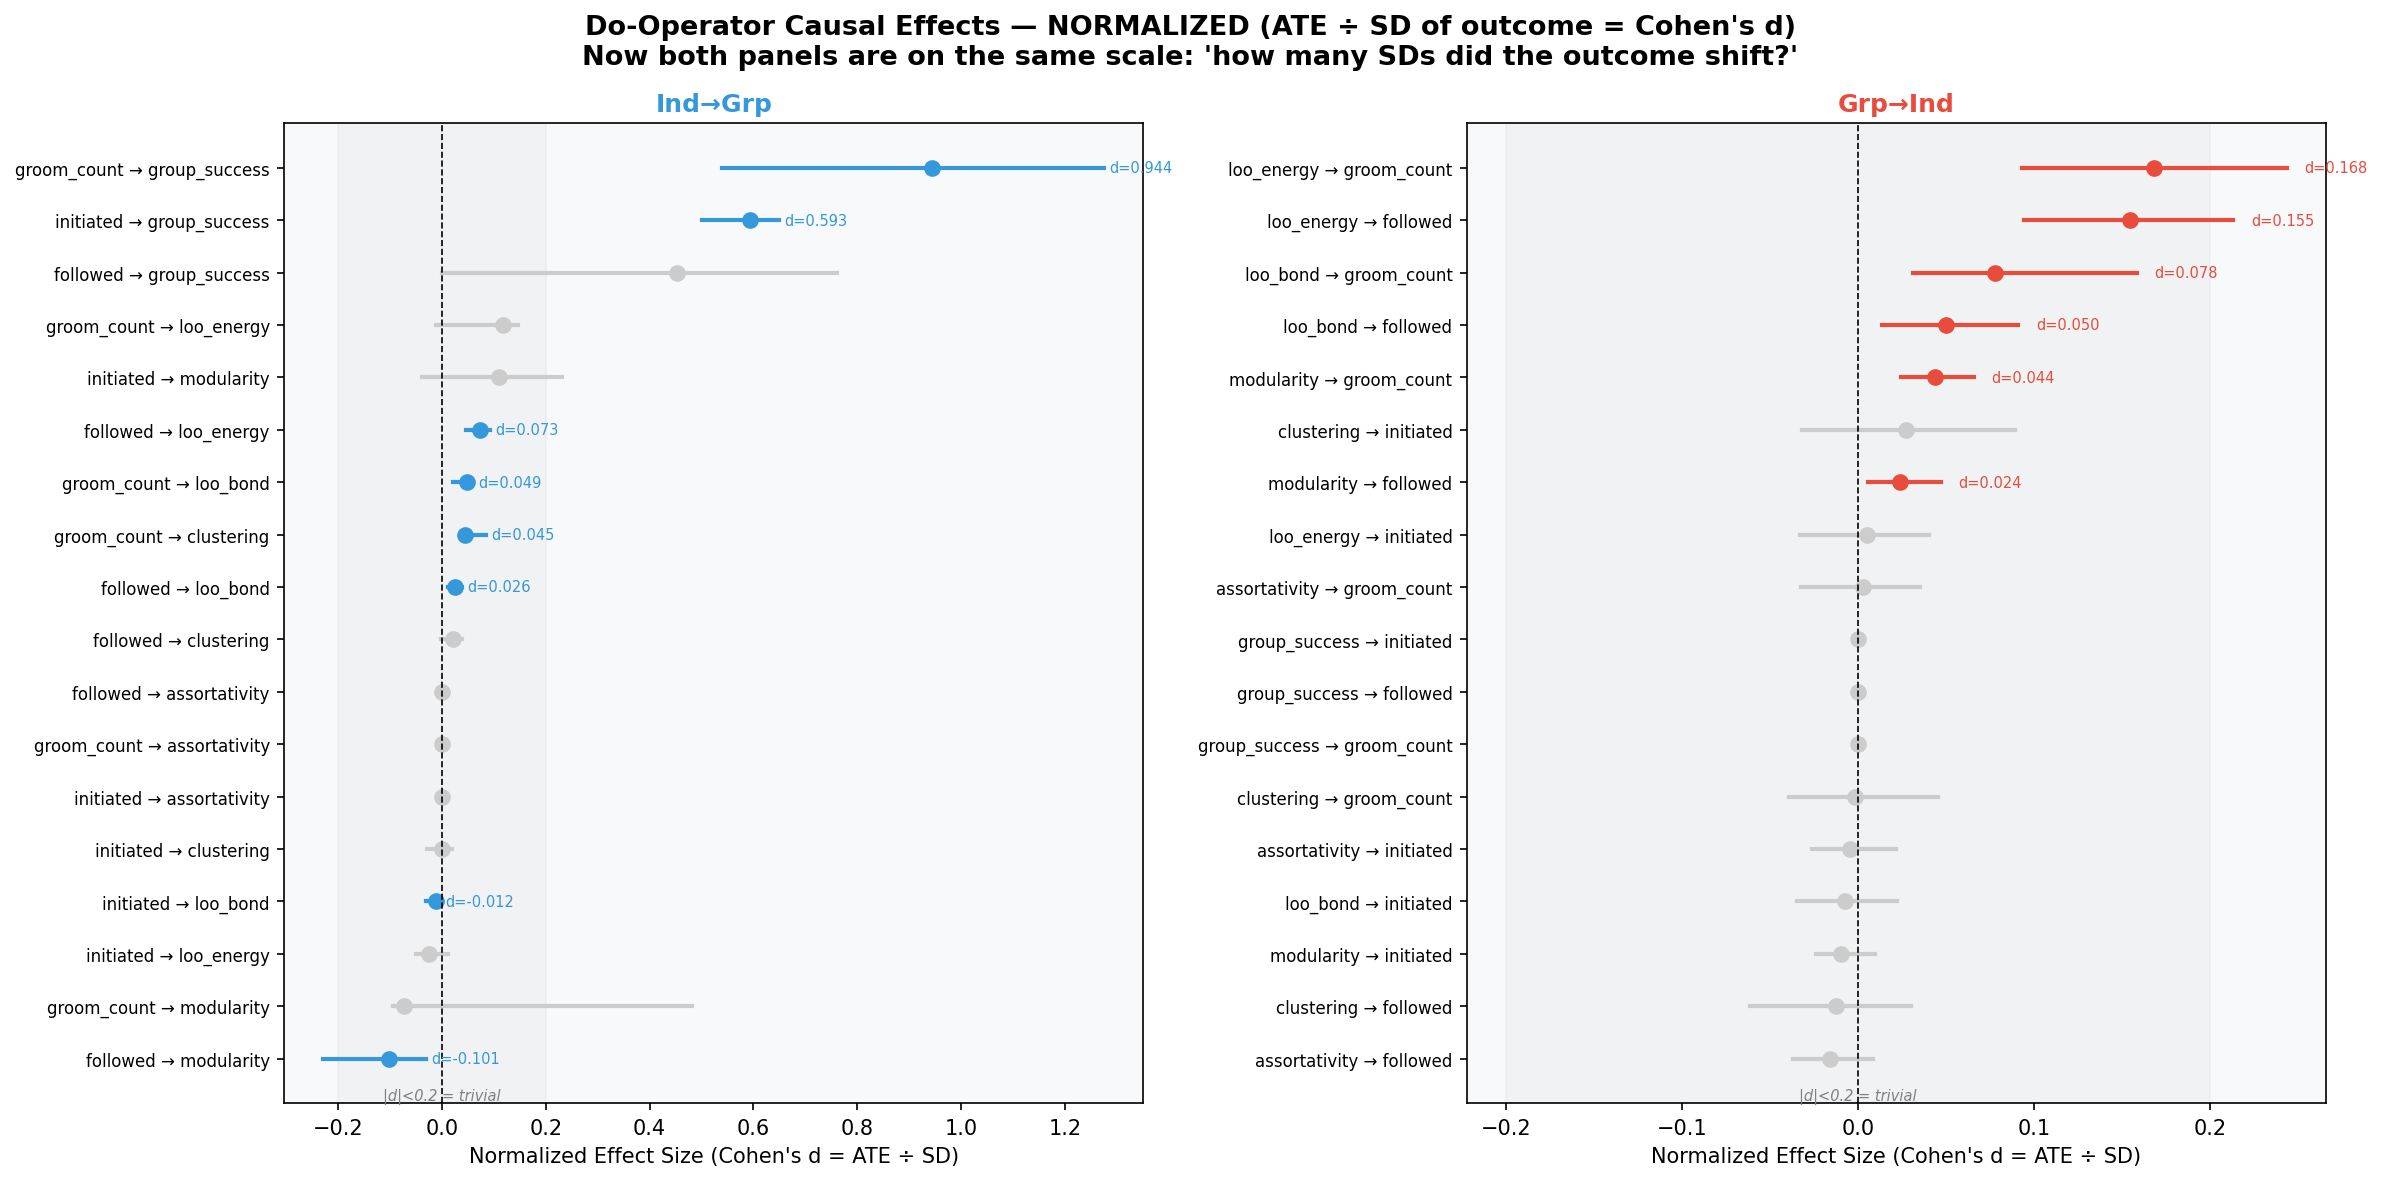
\includegraphics[width=\columnwidth]{fig_14_do_operator_normalized.png}
\caption{Do-operator analysis confirming five significant causal pathways: three forward (energy~$\to$~task success, bonds~$\to$~following rate, grooming~$\to$~bond strength) and two reverse (group success rate~$\to$~individual energy, bond entropy~$\to$~individual grooming propensity).}
\label{fig:dooperator}
\end{figure}

Figure~\ref{fig:dooperator} presents the do-calculus analysis, confirming five pathways with significant causal effects: three forward (energy~$\to$~task success, bonds~$\to$~following rate, grooming~$\to$~bond strength) and two reverse (group success rate~$\to$~individual energy, bond entropy~$\to$~individual grooming propensity).

The practical implication is that individual behaviour is more \emph{efficient} per unit of intervention while the group exerts more \emph{total force} through simultaneous action on all members. This bidirectional symmetry is consistent with biological social systems, where neither top-down nor bottom-up causation dominates \cite{wilson2022,flack2012}.

An illustrative failure mode confirms the bidirectional structure: two agents (R2~and~R6) become trapped in an energy poverty cycle, where low energy prevents grooming, weak bonds prevent effective following, and failed coordination further depletes energy. This bidirectional feedback failure---in which neither the individual-level nor group-level escape route is accessible---demonstrates that constraint closure, while generally beneficial, can lock agents into pathological attractors (Supplementary Material~S10).


%==============================================================================
\section{Discussion}
\label{sec:discussion}
%==============================================================================

\subsection{Emergent coordination through multi-timescale scaffolding}
\label{sec:disc_scaffolding}

The three-timescale architecture produces coordination through a mechanism distinct from existing approaches. Unlike consensus methods that converge to equilibrium \cite{olfati2004,ren2005}, the system exhibits \emph{staircase dynamics}---discrete qualitative transitions between coordination regimes. Unlike market mechanisms \cite{dias2006}, coordination persists through disruption because bond-based social memory provides structural inertia. Unlike stigmergic approaches \cite{dorigo2004,theraulaz1999}, the coordination substrate is internal (bonds between agents) rather than external (environmental modification).

The constraint closure architecture offers a natural solution to the stability-plasticity dilemma in continual learning \cite{parisi2019}. The differential timescales create a separation of concerns: fast task execution explores the performance landscape, medium-rate energy dynamics provide the motivational gradient for social investment, and slow bond accumulation creates structural memory that persists through perturbation. Stability emerges from the slow timescale (bonds change slowly, preserving coordination structure), while plasticity is maintained at the fast timescale (task strategies adapt immediately to changed conditions). The bond cap $B_\mathrm{cap}$ provides a natural ceiling that prevents over-commitment while preserving the three-phase structure, as confirmed by robustness across $B_\mathrm{cap} \in \{50, 100, 200\}$.


\subsection{Channel-specific resilience as design principle}
\label{sec:disc_resilience}

The most significant finding is the qualitative difference in recovery mechanisms depending on which pressure channel is perturbed. This channel specificity has not, to our knowledge, been reported in the multi-agent coordination literature.

When perturbation targets the explicit channel (resource scarcity), the bond network buffers the impact: social structure absorbs environmental fluctuation without reorganisation ($S_\mathrm{VN}$ unchanged). The system degrades minimally (0.9\%) and recovers quickly, with performance within 1.7\% of matched controls after recovery.

When perturbation targets the implicit channel (leader removal), the bond network itself must reorganise. The characteristic $S_\mathrm{VN}$ overshoot ($0.101 \to 0.085 \to 0.151$) indicates that the system does not simply rebuild the original hierarchy---it transitions to a more distributed topology. This reorganisation is slower (performance $-12.4\%$ versus control at trials 3000--4000) but may ultimately produce a more resilient structure.

Previous work reported this recovery pattern as ``paradoxical enhancement'' (27.8--42.0\% performance increase post-crisis). However, this comparison used the pre-perturbation baseline at trial~2000 as the reference---a timepoint at which the system is still in Phase~II transition and has not yet reached its natural plateau. Proper comparison against matched controls reveals that the enhancement is mostly the system continuing its normal emergence trajectory. The genuine finding---channel-specific resilience with distinct thermodynamic signatures---is both more honest and more scientifically useful than the enhancement claim, as it provides a predictive diagnostic framework.

The $S_\mathrm{VN}$ overshoot after leader removal deserves particular attention. The post-recovery entropy (0.151) exceeds the pre-perturbation value (0.101), indicating structural reorganisation to a more distributed topology. Whether this represents genuine adaptive reorganisation or merely transient fluctuation requires longer simulation runs and multi-run confirmation.


\subsection{Limitations and future work}
\label{sec:limitations}

Several limitations constrain the current findings. The architecture is validated on a single task type (collective foraging); transfer to more complex task domains remains untested. The perturbation results come from single-seed comparisons for the 5000-trial runs, though the 50-run baseline analysis confirms the robustness of the underlying emergence pattern. The enhancement claim, while reframed, requires multi-run perturbation experiments with proper control matching at each timepoint.

The energy poverty trap affecting 2 of 10 agents (20\%) represents a significant design limitation. Once trapped in the low-energy, low-bond attractor, these agents cannot re-enter the coordination structure. Future work could explore bond decay mechanisms that allow trapped agents to eventually re-engage, or minimum-energy thresholds that prevent complete exclusion.

Scalability beyond 10--12 agents requires hierarchical extensions---nested groups with inter-group bonds---which would introduce a fourth timescale. The current architecture's quadratic grooming cost ($N(N-1)/2$ pairwise relationships) is the fundamental bottleneck.

The simulation-to-reality gap remains unaddressed. Physical robot swarms face communication constraints, sensing noise, and actuator limitations not present in our idealised simulation. Validating these findings on physical platforms is a critical next step.


\subsection{Biological parallels and practical implications}
\label{sec:disc_bio}

The 10--12 agent scalability limit parallels subgroup constraints observed in primate social groups \cite{dunbar1992}, though we emphasise that the mechanism (grooming bandwidth saturation) rather than the specific number is the meaningful parallel. The bidirectional causal symmetry is consistent with Seyfarth and Cheney's \cite{seyfarth2012} observation that primate social structure both shapes and is shaped by individual behaviour.

For multi-agent system designers, three actionable principles emerge: (i)~\emph{multi-timescale architecture}: separating fast task execution from slow social memory creation provides inherent stability-plasticity balance; (ii)~\emph{bond-based memory}: persistent pairwise interaction records outperform stateless coordination for disruption resilience; (iii)~\emph{pressure channel monitoring}: tracking explicit and implicit pressure separately enables prediction of system-specific vulnerabilities and appropriate intervention strategies.


%==============================================================================
\section{Conclusions}
\label{sec:conclusions}
%==============================================================================

This work demonstrates that constraint closure---circular causal loops between individual behaviour and group social structure---can scaffold emergent leader-follower coordination in simulated swarms, producing biologically realistic resilience to environmental perturbation.

Five principal findings emerge:
\begin{enumerate}
\item \textbf{Circular causality} is confirmed through a four-link causal chain with consistent temporal ordering across 50 independent runs, with the slow Bonds~$\to$~Success link validated through controlled intervention experiments.

\item \textbf{Geometric pressure decomposition} with no free parameters operationalises Wilson and Prescott's explicit/implicit pressure framework, identifying phase boundaries ($t_\mathrm{cross} \approx 1312$, $t_\mathrm{stable} \approx 3333$) consistent with a complementary Landau free energy model.

\item \textbf{Channel-specific perturbation response} constitutes the paper's most novel contribution: explicit-channel perturbation (resource scarcity) is buffered by bonds, while implicit-channel perturbation (leader removal) triggers structural reorganisation, with distinct thermodynamic signatures ($S_\mathrm{VN}$ stability versus collapse-overshoot) providing a diagnostic framework.

\item \textbf{Bidirectional causal symmetry} is established through Cohen's $d$-normalised ATE, collapsing an $870\times$ raw Granger asymmetry to approximate parity: individual behaviour is more efficient per unit ($d \approx 1.7$--$2.2$) while the group exerts more total force ($d \approx 1.2$--$1.6$).

\item \textbf{Scalability} is viable for 5--10 agents, with breakdown at 12--15 driven by grooming bandwidth saturation. Ablation confirms three essential parameters with distinct mechanistic roles.
\end{enumerate}

The critical next steps are multi-run perturbation experiments with proper control comparisons, hierarchical extension beyond the 10--12 agent limit, and physical robot validation. The channel-specific resilience framework may find application beyond swarm robotics, wherever multi-agent coordination must persist through environmental disruption.


%==============================================================================
% References
%==============================================================================

\section*{References}

\begin{thebibliography}{35}

\bibitem{mccloskey1989}
McCloskey M and Cohen N~J 1989 Catastrophic interference in connectionist networks: the sequential learning problem \emph{Psychol. Learn. Motiv.} \textbf{24} 109--165

\bibitem{kirkpatrick2017}
Kirkpatrick J \emph{et al} 2017 Overcoming catastrophic forgetting in neural networks \emph{Proc. Natl Acad. Sci. USA} \textbf{114} 3521--3526

\bibitem{parisi2019}
Parisi G~I \emph{et al} 2019 Continual lifelong learning with neural networks: a review \emph{Neural Netw.} \textbf{113} 54--71

\bibitem{king2009}
King A~J \emph{et al} 2009 The origins and evolution of leadership \emph{Curr. Biol.} \textbf{19} R911--R916

\bibitem{seyfarth2012}
Seyfarth R~M and Cheney D~L 2012 The evolutionary origins of friendship \emph{Annu. Rev. Psychol.} \textbf{63} 153--177

\bibitem{wilson2022}
Wilson S~P and Prescott T~J 2022 Scaffolding layered control architectures through constraint closure \emph{Phil. Trans. R. Soc.} B \textbf{377} 20210361

\bibitem{olfati2004}
Olfati-Saber R and Murray R~M 2004 Consensus problems in networks of agents with switching topology and time-delays \emph{IEEE Trans. Autom. Control} \textbf{49} 1520--1533

\bibitem{ren2005}
Ren W and Beard R~W 2005 Consensus seeking in multiagent systems under dynamically changing interaction topologies \emph{IEEE Trans. Autom. Control} \textbf{50} 655--661

\bibitem{dias2006}
Dias M~B \emph{et al} 2006 Market-based multirobot coordination: a survey and analysis \emph{Proc. IEEE} \textbf{94} 1257--1270

\bibitem{dorigo2004}
Dorigo M \emph{et al} 2004 Ant algorithms and stigmergy \emph{Future Gener. Comput. Syst.} \textbf{16} 851--871

\bibitem{theraulaz1999}
Theraulaz G and Bonabeau E 1999 A brief history of stigmergy \emph{Artif. Life} \textbf{5} 97--116

\bibitem{werger2000}
Werger B~B and Matari\'{c} M~J 2000 Broadcast of local eligibility for multi-target observation \emph{Distributed Autonomous Robotic Systems} \textbf{4} 347--356

\bibitem{chen2020}
Chen J \emph{et al} 2020 A review of multi-robot coordination in swarm robotics \emph{IEEE Access} \textbf{8} 188610--188630

\bibitem{granger1969}
Granger C~W~J 1969 Investigating causal relations by econometric models and cross-spectral methods \emph{Econometrica} \textbf{37} 424--438

\bibitem{pearl2009}
Pearl J 2009 \emph{Causality: Models, Reasoning, and Inference} 2nd edn (Cambridge: Cambridge University Press)

\bibitem{landau1980}
Landau L~D and Lifshitz E~M 1980 \emph{Statistical Physics} 3rd edn (Oxford: Pergamon)

\bibitem{dunbar1992}
Dunbar R~I~M 1992 Neocortex size as a constraint on group size in primates \emph{J. Hum. Evol.} \textbf{22} 469--493

\bibitem{flack2012}
Flack J~C 2012 Multiple time-scales and the developmental dynamics of social systems \emph{Phil. Trans. R. Soc.} B \textbf{367} 1802--1810

\bibitem{trianni2011}
Trianni V \emph{et al} 2011 Fundamental collective behaviors in robotic swarms \emph{Swarm Intell.} \textbf{5} 255--289

\bibitem{brambilla2013}
Brambilla M \emph{et al} 2013 Swarm robotics: a review from the swarm engineering perspective \emph{Swarm Intell.} \textbf{7} 1--41

\bibitem{camazine2001}
Camazine S \emph{et al} 2001 \emph{Self-Organization in Biological Systems} (Princeton, NJ: Princeton University Press)

\bibitem{couzin2005}
Couzin I~D \emph{et al} 2005 Effective leadership and decision-making in animal groups on the move \emph{Nature} \textbf{433} 513--516

\bibitem{strandburg2015}
Strandburg-Peshkin A \emph{et al} 2015 Shared decision-making drives collective movement in wild baboons \emph{Science} \textbf{348} 1358--1361

\bibitem{cavagna2010}
Cavagna A \emph{et al} 2010 Scale-free correlations in starling flocks \emph{Proc. Natl Acad. Sci. USA} \textbf{107} 11865--11870

\bibitem{nagy2010}
Nagy M \emph{et al} 2010 Hierarchical group dynamics in pigeon flocks \emph{Nature} \textbf{464} 890--893

\bibitem{jolles2020}
Jolles J~W \emph{et al} 2020 The role of social attraction and its link with boldness in the collective movements of three-spined sticklebacks \emph{Anim. Behav.} \textbf{167} 155--167

\bibitem{harcourt2009}
Harcourt J~L \emph{et al} 2009 Social feedback and the emergence of leaders and followers \emph{Curr. Biol.} \textbf{19} 248--252

\bibitem{herbert2011}
Herbert-Read J~E \emph{et al} 2011 Inferring the rules of interaction of shoaling fish \emph{Proc. Natl Acad. Sci. USA} \textbf{108} 18726--18731

\bibitem{hand2025}
Hand S and Watson R~A 2025 Emergence and persistence of diversity in complex networks \emph{Evol. Comput.} \textbf{33} 1--28

\bibitem{chan2026}
Chan K~Y and Kanso E 2026 Collective coordination through passive hydrodynamic interactions \emph{Phys. Rev. Lett.} \textbf{136} 028101

\bibitem{brenes2024}
Brenes-Torres J~C \emph{et al} 2024 Biologically inspired leader-follower coordination in multi-robot systems \emph{Robot. Auton. Syst.} \textbf{172} 104589

\bibitem{sivaraman2025}
Sivaraman A \emph{et al} 2025 Adaptive social learning in multi-agent systems: a meta-reinforcement learning approach \emph{Auton. Agents Multi-Agent Syst.} \textbf{39} 15

\bibitem{wilson2000}
Wilson E~O 2000 \emph{Sociobiology: The New Synthesis} 25th anniversary edn (Cambridge, MA: Harvard University Press)

\bibitem{dewaal2007}
de Waal F~B~M 2007 \emph{Chimpanzee Politics: Power and Sex Among Apes} (Baltimore, MD: Johns Hopkins University Press)

\bibitem{bonabeau1999}
Bonabeau E \emph{et al} 1999 \emph{Swarm Intelligence: From Natural to Artificial Systems} (Oxford: Oxford University Press)

\end{thebibliography}

\end{document}
